\documentclass[11pt,oneside]{article}

\usepackage[a4paper,margin=26mm,headheight=15pt]{geometry}
\usepackage[T1]{fontenc}
\usepackage[utf8]{inputenc}
\IfFileExists{libertinus.sty}{\usepackage{libertinus}}{\usepackage{lmodern}}
\usepackage{microtype}
\usepackage{amsmath,amssymb,amsthm,mathtools,mathrsfs,bm}
\allowdisplaybreaks
\usepackage{booktabs,longtable,array,tabularx}
\usepackage{graphicx}
\usepackage{tikz}
\usetikzlibrary{arrows.meta,positioning,calc,decorations.pathreplacing}
\usepackage{pgfplots}
\pgfplotsset{compat=1.18}
\usepackage{xcolor}
\usepackage[most]{tcolorbox}
\usepackage{enumitem}
\usepackage{fancyhdr}
\usepackage{titlesec}
\usepackage{listings}
\usepackage{xurl}
\usepackage{hyperref}
\usepackage[nameinlink,noabbrev]{cleveref}

\definecolor{LinkBlue}{RGB}{28,77,132}
\definecolor{SoftBlue}{RGB}{236,244,251}
\definecolor{SoftGreen}{RGB}{239,247,239}
\definecolor{SoftAmber}{RGB}{252,247,232}
\definecolor{SoftGray}{RGB}{246,247,249}
\definecolor{RuleGray}{RGB}{190,198,207}
\definecolor{DeepGray}{RGB}{68,75,84}

\hypersetup{
  colorlinks=true,
  linkcolor=LinkBlue,
  citecolor=LinkBlue,
  urlcolor=LinkBlue,
  pdftitle={Fourier Decay of Rvachev's Up-Function: A Guided and Rigorous Account},
  pdfauthor={Vladimir Reshetnikov},
  pdfsubject={Exact dyadic renormalization, norm-dependent decay, fluctuations, Cesaro gauges, peaks, valleys, and integer-ratio generalizations},
  pdfkeywords={Rvachev up-function, Fabius function, sinc product, Fourier transform, Thue-Morse, transfer operator, lacunary product, asymptotic decay}
}

\pagestyle{fancy}
\fancyhf{}
\fancyhead[L]{\small Fourier decay of Rvachev's up-function}
\fancyhead[R]{\small\nouppercase{\rightmark}}
\fancyfoot[C]{\thepage}
\renewcommand{\headrulewidth}{0.4pt}

\titleformat{\section}{\Large\bfseries}{\thesection}{0.75em}{}
\titleformat{\subsection}{\large\bfseries}{\thesubsection}{0.7em}{}
\titleformat{\subsubsection}{\normalsize\bfseries}{\thesubsubsection}{0.7em}{}
\setcounter{secnumdepth}{3}
\setcounter{tocdepth}{2}
\setlength{\emergencystretch}{3em}
\setlist[itemize]{leftmargin=2em,itemsep=0.22em,topsep=0.35em}
\setlist[enumerate]{leftmargin=2.35em,itemsep=0.22em,topsep=0.35em}

\numberwithin{equation}{section}
\newtheorem{theorem}{Theorem}[section]
\newtheorem{proposition}[theorem]{Proposition}
\newtheorem{lemma}[theorem]{Lemma}
\newtheorem{corollary}[theorem]{Corollary}
\newtheorem{claim}[theorem]{Claim}
\theoremstyle{definition}
\newtheorem{definition}[theorem]{Definition}
\newtheorem{example}[theorem]{Example}
\theoremstyle{remark}
\newtheorem{remark}[theorem]{Remark}
\newtheorem{warning}[theorem]{Warning}

\crefname{theorem}{theorem}{theorems}
\Crefname{theorem}{Theorem}{Theorems}
\crefname{proposition}{proposition}{propositions}
\Crefname{proposition}{Proposition}{Propositions}
\crefname{lemma}{lemma}{lemmas}
\Crefname{lemma}{Lemma}{Lemmas}
\crefname{corollary}{corollary}{corollaries}
\Crefname{corollary}{Corollary}{Corollaries}
\crefname{definition}{definition}{definitions}
\Crefname{definition}{Definition}{Definitions}
\crefname{example}{example}{examples}
\Crefname{example}{Example}{Examples}
\crefname{remark}{remark}{remarks}
\Crefname{remark}{Remark}{Remarks}
\crefname{warning}{warning}{warnings}
\Crefname{warning}{Warning}{Warnings}

\newcommand{\R}{\mathbb R}
\newcommand{\C}{\mathbb C}
\newcommand{\N}{\mathbb N}
\newcommand{\Z}{\mathbb Z}
\newcommand{\e}{\mathrm e}
\newcommand{\ii}{\mathrm i}
\newcommand{\dd}{\,\mathrm d}
\newcommand{\abs}[1]{\left|#1\right|}
\newcommand{\norm}[1]{\left\lVert#1\right\rVert}
\newcommand{\floor}[1]{\left\lfloor#1\right\rfloor}
\newcommand{\ceil}[1]{\left\lceil#1\right\rceil}
\newcommand{\ind}{\mathbf 1}
\newcommand{\bigO}{\mathop{O}}
\newcommand{\littleo}{\mathop{o}}
\newcommand{\sinc}{\operatorname{sinc}}
\newcommand{\up}{\operatorname{up}}
\newcommand{\PhiUp}{\Phi}
\newcommand{\TM}{\tau}
\newcommand{\digitsum}{s_2}
\newcommand{\nuTwo}{\nu_2}
\newcommand{\Leb}{\operatorname{Leb}}
\newcommand{\Var}{\operatorname{Var}}
\newcommand{\Cov}{\operatorname{Cov}}
\newcommand{\Eop}{\mathbb E}
\newcommand{\Perron}{\mathcal P}
\newcommand{\Transfer}{\mathcal L}
\newcommand{\LambertW}{W}
\newcommand{\qpoch}[2]{\left(#1;#2\right)_{\!\infty}}
\newcommand{\defeq}{\mathrel{:=}}
\newcommand{\fourier}[1]{\widehat{#1}}

\newtcolorbox{guidebox}[1][]{
  enhanced,breakable,colback=SoftBlue,colframe=LinkBlue!55!black,
  boxrule=0.55pt,arc=1.5mm,left=1.2mm,right=1.2mm,top=1mm,bottom=1mm,
  fonttitle=\bfseries,title={Reading guide},#1}
\newtcolorbox{meaningbox}[1][]{
  enhanced,breakable,colback=SoftGreen,colframe=green!45!black,
  boxrule=0.55pt,arc=1.5mm,left=1.2mm,right=1.2mm,top=1mm,bottom=1mm,
  fonttitle=\bfseries,title={What the formula says},#1}
\newtcolorbox{statusbox}[1][]{
  enhanced,breakable,colback=SoftAmber,colframe=orange!55!black,
  boxrule=0.55pt,arc=1.5mm,left=1.2mm,right=1.2mm,top=1mm,bottom=1mm,
  fonttitle=\bfseries,title={Proof status},#1}
\newtcolorbox{pitfallbox}[1][]{
  enhanced,breakable,colback=SoftGray,colframe=DeepGray,
  boxrule=0.55pt,arc=1.5mm,left=1.2mm,right=1.2mm,top=1mm,bottom=1mm,
  fonttitle=\bfseries,title={Common pitfall},#1}

\lstdefinestyle{code}{
  basicstyle=\ttfamily\footnotesize,
  backgroundcolor=\color{SoftGray},
  frame=single,
  rulecolor=\color{RuleGray},
  columns=fullflexible,
  keepspaces=true,
  showstringspaces=false,
  breaklines=true,
  xleftmargin=0.7em,
  xrightmargin=0.7em,
  aboveskip=0.8em,
  belowskip=0.8em
}

\title{\bfseries Fourier Decay of Rvachev's Up-Function\\[0.35em]
\large A guided and rigorous account of exact products, decay spectra, fluctuations, Ces\`aro gauges, peaks, and valleys}
\author{Vladimir Reshetnikov\\[0.25em]\small Rewritten exposition for the \texttt{ProveIt} project}
\date{3 September 2026}

\begin{document}
\maketitle

\begin{abstract}
Let
\[
  \PhiUp(x)=\fourier{\up}(x)
  =\prod_{h=0}^{\infty}\sinc\!\left(\frac{\pi x}{2^h}\right),
  \qquad \sinc z=\begin{cases}\sin z/z,&z\ne0,\\1,&z=0.\end{cases}
\]
The transform is entire and decreases faster than every inverse power, but it has zeros at
all nonzero integers and its nonzero values fluctuate on many different scales.  Therefore
there is no single unqualified ``decay rate.''  The exact dyadic identity
\[
 \abs{\PhiUp(2^ny)}
 =\abs{\PhiUp(y)}\,\pi^{-n}y^{-n}2^{-n(n+1)/2}
   \prod_{j=1}^{n}\abs{\sin(\pi2^jy)}
\]
separates a deterministic log-normal factor from a lacunary dynamical product.  This
separation yields a spectrum of powers, according to whether size means a typical value,
an arithmetic mean, a root-mean-square value, or a uniform envelope.  With
\[
 E_\kappa(x)=x^{-\kappa}
   \exp\!\left(-\frac{(\log x)^2}{2\log2}\right),
\]
the four principal exponents are
\[
 \begin{aligned}
 \kappa_0&=3.151496129472318798\ldots,
 &\qquad \kappa_1&=2.748070014871332674\ldots,\\
 \kappa_2&=2.651496129472318798\ldots,
 &\qquad \kappa_\infty&=2.359014879111740707\ldots .
 \end{aligned}
\]
The first, third, and fourth have elementary closed forms; \(\kappa_1\) is determined by
the Perron root of an explicit weighted doubling operator and comes with a rigorous rational
enclosure.

The article gives detailed proofs of the product identities, zero multiplicities, unique
lobe maxima, exact dyadic renormalization, geometric-mean and almost-everywhere laws, exact
logarithmic variance, the martingale decomposition, the root-mean-square identity, the sharp
Gelfond envelope, Lambert--\(W\) boundary-layer asymptotics for dyadic-annulus maxima, and
explicit dyadic valley laws.  It also treats the arithmetic-mean/Ces\`aro problem: the natural
fixed gauge works shell-by-shell and at dyadic endpoints, a singular phase profile obstructs
an unrestricted limit for every bounded-distortion correction, and a deliberately
shell-adaptive positive analytic decreasing gauge does achieve the unrestricted limit.
Finally, the arguments are extended to products with an arbitrary integer geometric ratio.
Imported functional-analytic and probabilistic theorems are stated with their hypotheses,
and numerical evidence is kept visibly separate from exact proof.
\end{abstract}

\tableofcontents
\newpage

\section{What is being measured?}
\label{sec:introduction}

Rvachev's up-function is an even, nonnegative, compactly supported \(C^\infty\) function
on \([-1,1]\) with total mass one.  Under the Fourier convention
\begin{equation}
 \fourier f(\xi)=\int_{\R}f(t)\e^{-2\pi\ii t\xi}\dd t,
 \label{eq:fourier-convention}
\end{equation}
its transform is \(\PhiUp\) above.  The central question is deceptively simple:
\emph{how fast does \(\PhiUp(x)\) tend to zero?}

The first answer is that the question needs a qualifier.  Four facts force this.
\begin{enumerate}
\item \(\PhiUp(m)=0\) for every nonzero integer \(m\), so no positive function \(g\) can
      satisfy \(\abs{\PhiUp(x)}\sim g(x)\) on the entire real ray.
\item Between consecutive integers there is exactly one maximum of \(\abs{\PhiUp}\), but
      those maxima themselves have exceptional subsequences of very different sizes.
\item On a dyadic shell, the geometric mean, arithmetic mean, quadratic mean, and supremum
      of the oscillatory numerator grow at different exponential rates.
\item Even after the correct arithmetic-mean normalization is chosen, an incomplete final
      dyadic shell remembers its position within the shell.
\end{enumerate}

The universal part of the answer is the function
\begin{equation}
 E_\kappa(x)
 \defeq x^{-\kappa}\exp\!\left(-\frac{(\log x)^2}{2a}\right),
 \qquad a\defeq\log2,
 \qquad x>0.
 \label{eq:E-kappa}
\end{equation}
The coefficient \(1/(2\log2)\) is forced by the triangular product of dyadic denominators.
The power \(\kappa\), however, depends on how the remaining sine product is sampled.

\begin{guidebox}
The article has a short logical spine.
\begin{enumerate}
\item \Cref{sec:products} proves the exact product and zero structure.
\item \Cref{sec:dyadic} derives the master dyadic identity and explains the log-square term.
\item \Cref{sec:spectrum-overview,sec:typical,sec:transfer,sec:rms} obtain the four main
      exponents.
\item \Cref{sec:fluctuations} studies typical fluctuations beyond the leading exponent.
\item \Cref{sec:cesaro,sec:obstruction,sec:adaptive,sec:logmean} answer the additive and
      logarithmic averaging questions.
\item \Cref{sec:uniform,sec:annular,sec:valleys} describe large peaks, moving annular
      maxima, and deep exceptional valleys.
\item \Cref{sec:integer-base} gives the integer-ratio generalization.
\end{enumerate}
Readers interested only in the principal decay laws may read through \Cref{sec:rms}, then
jump to \Cref{sec:uniform} and the summary in \Cref{sec:conclusion}.
\end{guidebox}

\subsection{The four principal scales}

For \(q\in(0,\infty)\), let the normalized \(L^q\) size on the dyadic shell
\(D_n=[2^{n-1},2^n]\) be
\begin{equation}
 \mathcal M_{q,n}(H)
 =\left(\frac{1}{2^{n-1}}\int_{2^{n-1}}^{2^n}\abs{H(x)}^q\dd x\right)^{1/q}.
 \label{eq:shell-mean-intro}
\end{equation}
The endpoint conventions are the geometric mean \(q=0\) and the supremum \(q=\infty\).
The main scale dictionary is as follows.

\begin{center}
\small
\begin{tabularx}{\textwidth}{@{}>{\raggedright\arraybackslash}p{0.21\textwidth}
 >{\centering\arraybackslash}p{0.19\textwidth}
 >{\centering\arraybackslash}p{0.26\textwidth}X@{}}
\toprule
Notion of size & numerator rate & exponent in \(E_\kappa\) & interpretation\\
\midrule
Typical / geometric mean
 & \(1/2\)
 & \(\displaystyle\kappa_0=\frac32+\frac{\log\pi}{\log2}\)
 & Exact shell geometric mean; also the logarithmic rate on almost every fixed dyadic ray.\\[0.55em]
Arithmetic mean
 & \(\rho_1=0.6613226020\ldots\)
 & \(\displaystyle\kappa_1=\frac{\log\pi+\frac12\log2-\log\rho_1}{\log2}\)
 & Natural normalization for shell \(L^1\) means and ordinary Ces\`aro averages.\\[0.55em]
Root mean square
 & \(2^{-1/2}\)
 & \(\displaystyle\kappa_2=\frac{\log(2\pi)}{\log2}\)
 & Exact finite-level Parseval identity.\\[0.55em]
Uniform envelope
 & \(\sqrt3/2\)
 & \(\displaystyle\kappa_\infty=\frac32+\frac{\log(\pi/\sqrt3)}{\log2}\)
 & Sharp global pointwise upper bound, attained up to a fixed constant on a period-two ray.\\
\bottomrule
\end{tabularx}
\end{center}

Numerically,
\begin{equation}
 \begin{aligned}
 \kappa_\infty=2.3590148791\ldots
 &<\kappa_2=2.6514961295\ldots\\
 &<\kappa_1=2.7480700149\ldots
 <\kappa_0=3.1514961295\ldots .
 \end{aligned}
 \label{eq:kappa-order-intro}
\end{equation}
Larger \(q\) gives more weight to rare large values, so it produces slower decay and hence
a smaller exponent.

\begin{pitfallbox}
The power \(\log_2(2\pi)\) is neither an approximation nor a universally correct answer.
It is exactly the \emph{root-mean-square} exponent \(\kappa_2\).  The other notions of size
differ already by a nonzero power of \(x\); multiplying by \((\log x)^p\) cannot reconcile
them.
\end{pitfallbox}

\subsection{A compact statement of the final answer}

\begin{theorem}[Decay dictionary]
\label{thm:decay-dictionary}
Let \(E_\kappa\) be defined by \eqref{eq:E-kappa}.
\begin{enumerate}
\item For Lebesgue-almost every fixed \(y\in[1/2,1]\),
\[
 \abs{\PhiUp(2^ny)}=E_{\kappa_0}(2^ny)\e^{\littleo(n)}.
\]
The centered logarithm has asymptotic variance \(\pi^2/4\) per dyadic level and obeys the
central limit theorem and the law of the iterated logarithm stated in
\Cref{thm:clt-lil}.
\item For every fixed finite \(q>0\), there is \(A_q\in(0,\infty)\) such that
\[
 \mathcal M_{q,n}\!\left(\frac{\PhiUp}{E_{\kappa_q}}\right)\longrightarrow A_q,
\]
where \(\kappa_q\) is determined by the leading eigenvalue of the weighted transfer
operator in \Cref{sec:transfer}.
\item There is \(C<\infty\) such that
\[
 \abs{\PhiUp(x)}\le C E_{\kappa_\infty}(x),\qquad x\ge1,
\]
and this exponent is sharp on \(x=2^n(2/3)\).
\item The maximum on \([2^k,2^{k+1}]\), when compared with the envelope at the shell's left
endpoint, has the additional Lambert--\(W\) suppression of \Cref{thm:annular-main}.
\item The natural arithmetic-mean gauge \(A_1E_{\kappa_1}\) gives bounded ordinary Ces\`aro
means and convergence at dyadic endpoints.  At arbitrary endpoints it leaves a nonconstant
phase profile.  No bounded-distortion shell correction can remove that profile, but the
adaptive analytic gauge of \Cref{thm:analytic-adaptive} does give the unrestricted limit.
\item The fixed natural scale has an unrestricted limit under logarithmic rather than
additive averaging.
\end{enumerate}
\end{theorem}

The remainder of the article proves these statements in an order designed to make each new
object inevitable rather than mysterious.

\section{The entire product, its zeros, and its lobes}
\label{sec:products}

This section develops everything that can be obtained from elementary complex analysis and
real-variable calculus before any ergodic or spectral machinery enters.

\subsection{Normal convergence and three product representations}

\begin{proposition}[Entire convergence]
\label{prop:entire-convergence}
The infinite product
\begin{equation}
 \PhiUp(z)=\prod_{h=0}^{\infty}\sinc\!\left(\frac{\pi z}{2^h}\right)
 \label{eq:Phi-def}
\end{equation}
converges locally uniformly on \(\C\).  It defines an even entire function, real-valued on
\(\R\), with \(\PhiUp(0)=1\).
\end{proposition}

\begin{proof}
Fix a compact set \(K\subset\C\), and choose \(R\) with \(\abs z\le R\) on \(K\).  The
Taylor expansion at the origin is
\[
 \sinc w=1-\frac{w^2}{6}+O(w^4).
\]
Hence there are \(h_0\) and \(C_R\) such that, for \(h\ge h_0\) and \(z\in K\),
\[
 \abs{\sinc(\pi z/2^h)-1}\le C_R4^{-h}.
\]
The majorant \(\sum_{h\ge h_0}C_R4^{-h}\) converges.  The standard normal-convergence
criterion for infinite products therefore gives locally uniform convergence of the tail,
except possibly at zeros of a finite initial factor; multiplying by that finite prefix still
gives an entire limit.  Every factor is even, is real on the real axis, and equals one at
zero.  These properties pass to the locally uniform limit.
\end{proof}

There are two other representations that expose different structures.

\begin{theorem}[Cosine and zero-divisor products]
\label{thm:three-products}
For every \(z\in\C\),
\begin{equation}
 \boxed{
 \PhiUp(z)
 =\prod_{j=1}^{\infty}\cos^j\!\left(\frac{\pi z}{2^j}\right)
 =\prod_{m=1}^{\infty}\left(1-\frac{z^2}{m^2}\right)^{1+\nuTwo(m)}.}
 \label{eq:three-products}
\end{equation}
Both products converge locally uniformly.
\end{theorem}

\begin{proof}
The elementary double-angle identity gives, for every integer \(N\ge1\),
\[
 \sin t=2^N\sin(t/2^N)\prod_{j=1}^{N}\cos(t/2^j).
\]
After division by \(t\) and passage to the limit \(N\to\infty\), using
\(2^N\sin(t/2^N)/t\to1\), we obtain Vi\`ete's product
\[
 \sinc t=\prod_{j=1}^{\infty}\cos(t/2^j).
\]
Insert \(t=\pi z/2^h\) into \eqref{eq:Phi-def}.  The factor
\(\cos(\pi z/2^j)\) occurs once for every pair \((h,r)\) with \(h\ge0\), \(r\ge1\), and
\(h+r=j\); there are exactly \(j\) such pairs.  Local absolute convergence of the
logarithms away from zeros, followed by analytic continuation across the discrete zero set,
justifies the regrouping and proves the first equality.

For the second equality use Euler's sine product
\[
 \sinc(\pi w)=\prod_{\ell=1}^{\infty}\left(1-\frac{w^2}{\ell^2}\right).
\]
At level \(h\), the zero factors are
\(1-z^2/(2^h\ell)^2\).  A fixed positive integer \(m\) occurs once for each representation
\(m=2^h\ell\), equivalently for each \(0\le h\le\nuTwo(m)\); its multiplicity is therefore
\(1+\nuTwo(m)\).  On any compact set,
\[
 \sum_{h\ge0}\sum_{\ell\ge1}\frac{\abs z^2}{4^h\ell^2}<\infty,
\]
so the double product is normally convergent and may be rearranged.  This proves the second
equality.
\end{proof}

\subsection{Scaling, zeros, and local zero coefficients}

The product immediately implies the one-step relations
\begin{equation}
 \PhiUp(2x)=\sinc(2\pi x)\PhiUp(x),
 \qquad
 \PhiUp(x)=\sinc(\pi x)\PhiUp(x/2).
 \label{eq:one-step}
\end{equation}
The first is obtained by separating the \(h=0\) factor from \(\PhiUp(2x)\); the second is
the same identity with \(x\) replaced by \(x/2\).

\begin{proposition}[Integer zeros and their exact orders]
\label{prop:zeros}
The nonzero zeros of \(\PhiUp\) are precisely the nonzero integers.  At
\(m\in\Z\setminus\{0\}\), the multiplicity is
\begin{equation}
 d(m)=1+\nuTwo(\abs m).
 \label{eq:zero-order}
\end{equation}
If \(b\ge1\) is an integer, \(d=1+\nuTwo(b)\), and \(z\uparrow b\), then
\begin{equation}
 \abs{\PhiUp(z)}
 =b^{-d}\abs{\PhiUp(b/2^d)}(b-z)^d\bigl(1+O(b-z)\bigr).
 \label{eq:local-zero}
\end{equation}
\end{proposition}

\begin{proof}
The last product in \eqref{eq:three-products} shows both the zero set and the multiplicity.
For the coefficient, return to the sinc product.  Exactly the factors with
\(0\le h\le d-1\) vanish at \(z=b\).  Each zero is simple, and direct differentiation gives
\[
 \left|\frac{\dd}{\dd z}\sinc\!\left(\frac{\pi z}{2^h}\right)\bigg|_{z=b}\right|
 =\frac1b.
\]
Thus the product of the \(d\) vanishing factors contributes
\(b^{-d}(b-z)^d(1+O(b-z))\).  The remaining factors are nonzero at \(b\) and their value is
\[
 \prod_{h=d}^{\infty}\left|\sinc\!\left(\frac{\pi b}{2^h}\right)\right|
 =\abs{\PhiUp(b/2^d)}.
\]
Multiplying the two parts proves \eqref{eq:local-zero}.
\end{proof}

\subsection{Exactly one extremum in every unit interval}

The zero-divisor product does more than locate zeros: its logarithm is strictly concave
between consecutive zeros.

\begin{theorem}[Strict logarithmic concavity and unique lobe maxima]
\label{thm:unique-lobe}
The function \(\PhiUp\) is positive and strictly decreasing on \((0,1)\).  For every
integer \(m\ge1\), the function \(\abs{\PhiUp}\) has exactly one critical point
\(\xi_m\in(m,m+1)\), and this point is the strict maximum on that interval.  Moreover,
\begin{equation}
 \operatorname{sgn}\PhiUp(x)=(-1)^{\digitsum(m)},
 \qquad m<x<m+1,
 \label{eq:lobe-sign}
\end{equation}
where \(\digitsum(m)\) is the number of ones in the binary expansion of \(m\).
\end{theorem}

\begin{proof}
Fix a compact subinterval avoiding the integers.  Since
\(\sum_{k\ge1}(1+\nuTwo(k))/k^2<\infty\), the logarithm of the last product in
\eqref{eq:three-products} may be differentiated term by term.  We obtain
\begin{align}
 \frac{\dd}{\dd x}\log\abs{\PhiUp(x)}
 &=-2x\sum_{k=1}^{\infty}\frac{1+\nuTwo(k)}{k^2-x^2},
 \label{eq:log-derivative}\\
 \frac{\dd^2}{\dd x^2}\log\abs{\PhiUp(x)}
 &=-2\sum_{k=1}^{\infty}(1+\nuTwo(k))
   \frac{k^2+x^2}{(k^2-x^2)^2}<0.
 \label{eq:log-concavity}
\end{align}
For \(0<x<1\), every denominator in \eqref{eq:log-derivative} is positive, hence the
logarithmic derivative is negative.  This proves strict decrease on the central lobe.

Now fix \(m\ge1\).  Equation \eqref{eq:log-concavity} says that the logarithmic derivative
is strictly decreasing on \((m,m+1)\).  The term \(k=m\) forces it to tend to \(+\infty\)
as \(x\downarrow m\), while the term \(k=m+1\) forces it to tend to \(-\infty\) as
\(x\uparrow m+1\).  The intermediate value theorem and strict monotonicity give exactly one
zero.  Strict log-concavity makes that zero the unique maximum of the modulus.

It remains to compute the sign.  Starting from the positive central lobe, crossing the zero
at \(k\) changes the sign \(1+\nuTwo(k)\) times.  Therefore the sign on \((m,m+1)\) is
\[
 (-1)^{\sum_{k=1}^{m}(1+\nuTwo(k))}
 =(-1)^{m+\nuTwo(m!)}.
\]
Legendre's formula in base two is \(\nuTwo(m!)=m-\digitsum(m)\).  Hence the exponent is
\(2m-\digitsum(m)\), which has the same parity as \(\digitsum(m)\).  This proves
\eqref{eq:lobe-sign}.
\end{proof}

\begin{meaningbox}
The graph is not irregular in the small: every interval \((m,m+1)\) contains one clean,
strictly log-concave lobe.  The irregularity is in the \emph{heights and locations} of those
lobes as \(m\) ranges through integers with different binary structure.
\end{meaningbox}

\subsection{Reciprocal Gamma and corrected \texorpdfstring{\(q\)}{q}-Pochhammer tails}

These factorizations are useful for local evaluation and for separating finitely many nearby
zeros from a rapidly convergent analytic tail.

\begin{theorem}[Gamma product]
\label{thm:gamma-product}
For every \(z\in\C\),
\begin{equation}
 \PhiUp(z)=\prod_{n=0}^{\infty}
 \frac{1}{\Gamma(1+z/2^n)\Gamma(1-z/2^n)}.
 \label{eq:gamma-product}
\end{equation}
\end{theorem}

\begin{proof}
Euler's reflection formula and \(\Gamma(1+w)=w\Gamma(w)\) imply
\[
 \Gamma(1+w)\Gamma(1-w)=\frac{\pi w}{\sin\pi w},
\]
so its reciprocal is \(\sinc(\pi w)\).  Substitute \(w=z/2^n\) and multiply over
\(n\ge0\).  Local uniform convergence follows from the same \(1+O(4^{-n})\) estimate as in
\Cref{prop:entire-convergence}.
\end{proof}

For \(\abs q<1\), write
\[
 (u;q)_\infty=\prod_{j=0}^{\infty}(1-uq^j),
 \qquad
 c_k=\frac{\zeta(2k)-1}{k}>0.
\]

\begin{theorem}[Zero-extracted Pochhammer tail]
\label{thm:pochhammer-tail}
For an integer \(m\ge0\), define
\[
 R_m(z)=\prod_{n=m}^{\infty}\sinc\!\left(\frac{\pi z}{2^n}\right).
\]
If \(\abs z<2^{m+1}\), then
\begin{equation}
 \boxed{
 R_m(z)
 =\qpoch{z^2/4^m}{1/4}
 \exp\!\left[-\sum_{k=1}^{\infty}
  \frac{c_k}{1-4^{-k}}\left(\frac{z}{2^m}\right)^{2k}\right].}
 \label{eq:pochhammer-tail}
\end{equation}
Consequently,
\begin{equation}
 \PhiUp(z)=\left(\prod_{n=0}^{m-1}
 \sinc\!\left(\frac{\pi z}{2^n}\right)\right)R_m(z),
 \label{eq:prefix-tail}
\end{equation}
with the empty prefix interpreted as one.
\end{theorem}

\begin{proof}
Euler's sine product gives, for \(\abs w<2\),
\begin{align*}
 \sinc(\pi w)
 &=(1-w^2)\prod_{\ell=2}^{\infty}
       \left(1-\frac{w^2}{\ell^2}\right),\\
 \log\frac{\sinc(\pi w)}{1-w^2}
 &=\sum_{\ell=2}^{\infty}\log\left(1-\frac{w^2}{\ell^2}\right).
\end{align*}
The double series obtained from \(\log(1-u)=-\sum_{k\ge1}u^k/k\) is absolutely
convergent when \(\abs w<2\).  Interchanging sums gives
\[
 \log\frac{\sinc(\pi w)}{1-w^2}
 =-\sum_{k=1}^{\infty}\frac{w^{2k}}{k}
   \sum_{\ell=2}^{\infty}\ell^{-2k}
 =-\sum_{k=1}^{\infty}c_kw^{2k}.
\]
Thus
\begin{equation}
 \sinc(\pi w)=(1-w^2)
 \exp\!\left(-\sum_{k=1}^{\infty}c_kw^{2k}\right),
 \qquad \abs w<2.
 \label{eq:local-sinc-factor}
\end{equation}
Apply \eqref{eq:local-sinc-factor} with \(w=z/2^n\) and multiply over \(n\ge m\).  The
condition \(\abs z<2^{m+1}\) places every factor inside the common disk of convergence.  The
algebraic factors give
\[
 \prod_{n=m}^{\infty}\left(1-\frac{z^2}{4^n}\right)
 =\left(z^2/4^m;1/4\right)_\infty.
\]
For the exponent, absolute convergence allows us to interchange the \(n\)- and \(k\)-sums:
\begin{align*}
 -\sum_{n=m}^{\infty}\sum_{k=1}^{\infty}c_k\frac{z^{2k}}{4^{nk}}
 &=-\sum_{k=1}^{\infty}c_kz^{2k}
   \frac{4^{-mk}}{1-4^{-k}}\\
 &=-\sum_{k=1}^{\infty}\frac{c_k}{1-4^{-k}}
   \left(\frac{z}{2^m}\right)^{2k}.
\end{align*}
This proves \eqref{eq:pochhammer-tail}; splitting the defining product at \(m\) proves
\eqref{eq:prefix-tail}.
\end{proof}

\begin{pitfallbox}
The disk \(\abs z<2^{m+1}\) is the convergence disk of the chosen logarithmic expansion
after extracting only the nearest zero pair.  It is not the support of \(\PhiUp\), and it
does not imply that \(\PhiUp\) vanishes outside the disk.  For a larger \(z\), increase
\(m\), extract more zero layers, or analytically continue the formula.
\end{pitfallbox}

\section{Exact dyadic renormalization}
\label{sec:dyadic}

All large-argument results in this article begin with one exact identity.  It converts the
infinite sinc product at a large point into a fixed compact ``mantissa'' factor and a finite
lacunary sine product.

\subsection{The master factorization}

Let
\begin{equation}
 T(t)=2t\pmod1,
 \qquad s(t)=\abs{\sin(\pi t)},
 \qquad
 B_n(y)=\prod_{j=1}^{n}s(T^jy)
       =\prod_{j=1}^{n}\abs{\sin(\pi2^jy)}.
 \label{eq:T-s-B}
\end{equation}

\begin{theorem}[Exact dyadic factorization]
\label{thm:dyadic-factorization}
For every integer \(n\ge1\) and every \(y\in[1/2,1]\),
\begin{equation}
 \boxed{
 \abs{\PhiUp(2^ny)}
 =\abs{\PhiUp(y)}\,\pi^{-n}y^{-n}2^{-n(n+1)/2}B_n(y).}
 \label{eq:dyadic-factorization}
\end{equation}
For a real \(\kappa\), define the compact phase factor
\begin{equation}
 W_\kappa(y)
 =\abs{\PhiUp(y)}y^\kappa
   \exp\!\left(\frac{(\log y)^2}{2a}\right),
 \qquad a=\log2.
 \label{eq:W-kappa}
\end{equation}
Then
\begin{equation}
 \boxed{
 \frac{\abs{\PhiUp(2^ny)}}{E_\kappa(2^ny)}
 =W_\kappa(y)
   \exp\!\bigl(n(\kappa a-\log\pi-a/2)\bigr)B_n(y).}
 \label{eq:master-normalization}
\end{equation}
\end{theorem}

\begin{proof}
Iterating the first identity in \eqref{eq:one-step} gives
\[
 \PhiUp(2^ny)=\PhiUp(y)\prod_{j=1}^{n}\sinc(\pi2^jy).
\]
Taking absolute values separates each sinc factor into its numerator and denominator:
\[
 \left|\sinc(\pi2^jy)\right|
 =\frac{\abs{\sin(\pi2^jy)}}{\pi2^jy}.
\]
The product of the numerators is \(B_n(y)\).  The product of the denominators is
\[
 \prod_{j=1}^{n}(\pi2^jy)
 =\pi^ny^n2^{1+2+\cdots+n}
 =\pi^ny^n2^{n(n+1)/2}.
\]
This proves \eqref{eq:dyadic-factorization}.

To derive the normalized identity, put \(L=\log(2^ny)=na+\log y\).  Dividing by
\(E_\kappa(2^ny)=\exp(-L^2/(2a)-\kappa L)\) adds
\[
 \frac{L^2}{2a}+\kappa L
 =\frac{a}{2}n^2+n\log y+\frac{(\log y)^2}{2a}
   +\kappa an+\kappa\log y
\]
to the logarithm.  The term \(n\log y\) cancels the factor \(y^{-n}\), and
\(an^2/2\) cancels the quadratic part of \(-a n(n+1)/2\), leaving \(-an/2\).
The remaining terms are exactly \eqref{eq:master-normalization}.
\end{proof}

\subsection{Where the log-normal factor comes from}

The origin of the leading decay can now be seen without any probability theory.  The
triangular denominator contributes
\[
 2^{-n(n+1)/2}
 =\exp\!\left(-\frac{a}{2}n^2-\frac{a}{2}n\right).
\]
Since \(x=2^ny\) with \(y\in[1/2,1]\), one has
\(n=(\log x-\log y)/a\).  Substituting this into the quadratic term gives
\begin{equation}
 -\frac{a}{2}n^2
 =-\frac{(\log x)^2}{2a}
   +\frac{\log x\log y}{a}
   -\frac{(\log y)^2}{2a}.
 \label{eq:triangular-to-log-square}
\end{equation}
The mixed term is canceled by \(y^{-n}\), exactly as in the proof above.  Thus
\(- (\log x)^2/(2\log2)\) is deterministic and unavoidable.  The remaining finite product
\(B_n(y)\) decides only the coefficient of the linear term in \(n\), hence the power of
\(x\), together with smaller fluctuations.

\begin{center}
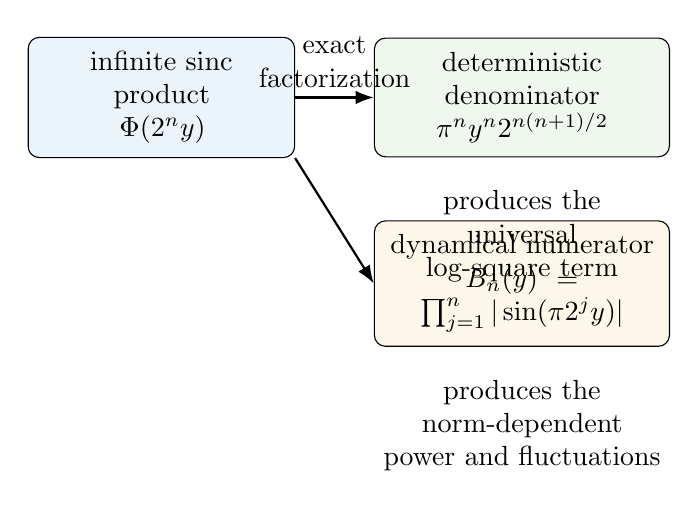
\begin{tikzpicture}[node distance=8mm and 10mm,>=Latex]
\node[draw,rounded corners,fill=SoftBlue,inner sep=5pt,text width=.25\textwidth,align=center]
 (prod) {infinite sinc product\\\(\PhiUp(2^ny)\)};
\node[draw,rounded corners,fill=SoftGreen,inner sep=5pt,text width=.28\textwidth,align=center,
 right=of prod] (det) {deterministic denominator\\
 \(\pi^ny^n2^{n(n+1)/2}\)};
\node[draw,rounded corners,fill=SoftAmber,inner sep=5pt,text width=.28\textwidth,align=center,
 below=of det] (dyn) {dynamical numerator\\
 \(B_n(y)=\prod_{j=1}^n|\sin(\pi2^jy)|\)};
\draw[->,thick] (prod) -- node[above,align=center]{exact\\factorization} (det);
\draw[->,thick] (prod.south east) -- (dyn.west);
\node[below=3mm of det,text width=.27\textwidth,align=center] {produces the universal\\log-square term};
\node[below=3mm of dyn,text width=.29\textwidth,align=center] {produces the norm-dependent\\power and fluctuations};
\end{tikzpicture}
\end{center}

\begin{meaningbox}
The difficult-looking entire function has been reduced to a familiar dynamical system: the
doubling map on the circle.  Different statistical questions about \(\PhiUp\) become
different statistical questions about the same cocycle \(\log|\sin(\pi t)|\).
\end{meaningbox}

\subsection{The Thue--Morse polynomial hidden in the numerator}

Let
\[
 \TM_k=(-1)^{\digitsum(k)},
\]
the signed Thue--Morse sequence.  Define
\begin{equation}
 P_n(t)=\prod_{j=0}^{n-1}\left(1-\e^{2\pi\ii2^jt}\right).
 \label{eq:TM-product}
\end{equation}

\begin{proposition}[Finite Thue--Morse expansion]
\label{prop:TM-polynomial}
For every integer \(n\ge0\),
\begin{equation}
 P_n(t)=\sum_{k=0}^{2^n-1}\TM_k\e^{2\pi\ii kt},
 \qquad
 \abs{P_n(t)}=2^n\prod_{j=0}^{n-1}s(T^jt).
 \label{eq:TM-expansion}
\end{equation}
\end{proposition}

\begin{proof}
The statement is immediate for \(n=0\).  Assume the expansion for \(n\).  Then
\begin{align*}
 P_{n+1}(t)
 &=P_n(t)\left(1-\e^{2\pi\ii2^nt}\right)\\
 &=\sum_{k=0}^{2^n-1}\TM_k\e^{2\pi\ii kt}
   -\sum_{k=0}^{2^n-1}\TM_k\e^{2\pi\ii(k+2^n)t}.
\end{align*}
The binary digit identities
\(\TM_k=(-1)^{\digitsum(k)}\) and
\(\TM_{k+2^n}=-\TM_k\) show that the two sums combine into the claimed expansion for
\(n+1\).  Finally,
\(
 |1-\e^{2\pi\ii u}|=2|\sin\pi u|
\), so taking moduli in \eqref{eq:TM-product} gives the second formula.
\end{proof}

Thus the numerator in the Fourier decay problem is, up to a power of two, the modulus of a
classical Thue--Morse trigonometric polynomial.  Parseval, Gelfond's supremum estimate, Riesz
products, and thermodynamic formalism are all available because of this exact bridge.

For completeness we also record the finite product-to-sum identity that motivated the
original investigation.

\begin{proposition}[Finite sinc product as a Thue--Morse sine sum]
\label{prop:finite-sinc-sum}
For every integer \(m\ge0\) and every real \(x\ne0\),
\begin{equation}
 \prod_{h=0}^{m}\sinc\!\left(\frac{\pi x}{2^h}\right)
 =\frac{2^{m(m-1)/2}}{(\pi x)^{m+1}}
 \sum_{r=0}^{2^m-1}\TM_r
 \sin\!\left(\frac{\pi m}{2}+\frac{(2r+1)\pi x}{2^m}\right).
 \label{eq:finite-sinc-sum}
\end{equation}
At \(x=0\), both sides have the continuous value one.
\end{proposition}

\begin{proof}
Put \(\theta=\pi x/2^m\).  Reversing the order of factors gives
\[
 \prod_{h=0}^{m}\sin\!\left(\frac{\pi x}{2^h}\right)
 =\prod_{j=0}^{m}\sin(2^j\theta).
\]
Apply \Cref{prop:TM-polynomial} with \(m+1\) factors and use
\[
 1-\e^{2\ii u}=-2\ii\e^{\ii u}\sin u.
\]
After solving for the product of sines, pair the term indexed by \(r\) with the term indexed
by \(2^{m+1}-1-r\).  Binary complementation gives
\(
 \TM_{2^{m+1}-1-r}=(-1)^{m+1}\TM_r
\), and taking the appropriate real or imaginary part yields
\[
 \prod_{j=0}^{m}\sin(2^j\theta)
 =2^{-m}\sum_{r=0}^{2^m-1}\TM_r
   \sin\!\left(\frac{\pi m}{2}+(2r+1)\theta\right).
\]
The product of the sinc denominators is
\[
 \prod_{h=0}^{m}\frac{\pi x}{2^h}
 =\frac{(\pi x)^{m+1}}{2^{m(m+1)/2}}.
\]
Dividing the two formulas proves \eqref{eq:finite-sinc-sum}.  Continuity at zero follows
from the original product.
\end{proof}

\section{One product, many notions of size}
\label{sec:spectrum-overview}

The master identity reduces the choice of a decay exponent to one question: what is the
exponential growth rate of \(B_n\) under the chosen functional?

For \(q\in(0,\infty)\), define
\begin{equation}
 \mathcal M_{q,n}(H)
 =\left(2\int_{1/2}^{1}\abs{H(2^ny)}^q\dd y\right)^{1/q}.
 \label{eq:shell-Lq}
\end{equation}
This is identical to \eqref{eq:shell-mean-intro} after \(x=2^ny\).  The endpoint cases are
\begin{align}
 \mathcal M_{0,n}(H)
 &=\exp\!\left(2\int_{1/2}^{1}\log\abs{H(2^ny)}\dd y\right),
 \label{eq:shell-L0}\\
 \mathcal M_{\infty,n}(H)
 &=\sup_{1/2\le y\le1}\abs{H(2^ny)}.
 \label{eq:shell-Linf}
\end{align}
Zeros cause no difficulty in \eqref{eq:shell-L0} because logarithmic singularities are
locally integrable.

Suppose, heuristically for the moment, that the chosen size of \(B_n\) behaves like
\(\Lambda^n\).  In \eqref{eq:master-normalization}, the \(n\)-dependent exponential then
has rate
\[
 \kappa a-\log\pi-a/2+\log\Lambda.
\]
To make the normalized size neither vanish nor blow up, we must set
\begin{equation}
 \boxed{
 \kappa(\Lambda)=\frac{\log\pi+a/2-\log\Lambda}{a}.}
 \label{eq:kappa-from-Lambda}
\end{equation}
Every exponent in the article is an instance of this one formula.

\begin{center}
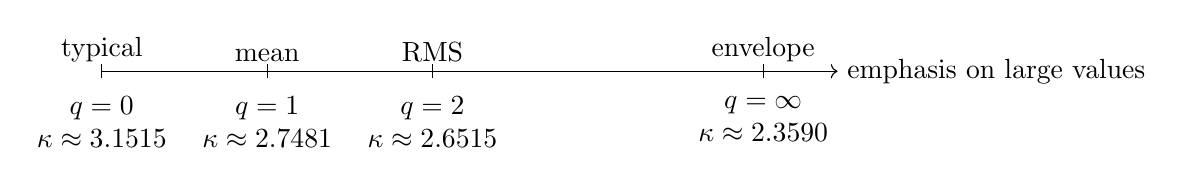
\begin{tikzpicture}[x=2.1cm,y=1.1cm]
\draw[->] (0,0) -- (4.45,0) node[right]{emphasis on large values};
\foreach \x/\lab/\num in {0/$q=0$/3.1515,1/$q=1$/2.7481,2/$q=2$/2.6515,4/$q=\infty$/2.3590}{
  \draw (\x,0.08)--(\x,-0.08) node[below=3pt,align=center]{\lab\\$\kappa\approx\num$};}
\node[above] at (0,0) {typical};
\node[above] at (1,0) {mean};
\node[above] at (2,0) {RMS};
\node[above] at (4,0) {envelope};
\end{tikzpicture}
\end{center}

The next four sections make the heuristic precise.  The geometric-mean and RMS cases admit
particularly elementary exact proofs.  The general finite-\(q\) case is governed by a
weighted transfer operator, and the supremum case is governed by an optimizing periodic
orbit.

\section{Geometric-mean and almost-everywhere decay}
\label{sec:typical}

The \(q=0\) endpoint is elementary because Lebesgue measure is invariant under doubling and
because the mean logarithm of the sine is known exactly.

\begin{lemma}[The log-sine integral]
\label{lem:log-sine}
One has
\begin{equation}
 \int_0^1\log\abs{\sin(\pi t)}\dd t=-\log2=-a.
 \label{eq:log-sine}
\end{equation}
\end{lemma}

\begin{proof}
Let \(I=\int_0^{\pi/2}\log(\sin u)\dd u\).  By \(u\mapsto\pi/2-u\), the same integral
is \(\int_0^{\pi/2}\log(\cos u)\dd u\).  Hence
\begin{align*}
 2I
 &=\int_0^{\pi/2}\log(\sin u\cos u)\dd u\\
 &=\int_0^{\pi/2}\log\!\left(\frac12\sin2u\right)\dd u
 =-\frac{\pi}{2}\log2+\frac12\int_0^\pi\log(\sin v)\dd v.
\end{align*}
Symmetry gives \(\int_0^\pi\log(\sin v)\dd v=2I\), so
\(I=-(\pi/2)\log2\).  Rescaling and using symmetry once more gives
\eqref{eq:log-sine}.
\end{proof}

\begin{theorem}[Exact shell geometric mean]
\label{thm:geometric-mean}
Set
\begin{equation}
 \boxed{\kappa_0=\frac32+\frac{\log\pi}{a}}
 =3.151496129472318798\ldots .
 \label{eq:kappa0}
\end{equation}
Then, for every \(n\ge1\),
\begin{equation}
 \mathcal M_{0,n}\!\left(\frac{\PhiUp}{E_{\kappa_0}}\right)
 =\exp\!\left(2\int_{1/2}^{1}\log W_{\kappa_0}(y)\dd y\right).
 \label{eq:exact-geometric-mean}
\end{equation}
In particular, the normalized shell geometric mean is exactly independent of \(n\).
\end{theorem}

\begin{proof}
Take logarithms in \eqref{eq:master-normalization}, multiply by two, and integrate over
\(y\in[1/2,1]\).  Put \(z=2y-1\).  For \(j\ge1\),
\(T^jy=T^{j-1}z\), and \(2\dd y=\dd z\).  Since Lebesgue measure is invariant under
\(T\), \Cref{lem:log-sine} gives
\[
 2\int_{1/2}^{1}\log B_n(y)\dd y
 =\sum_{j=1}^{n}\int_0^1\log s(T^{j-1}z)\dd z=-na.
\]
For \(\kappa=\kappa_0\),
\[
 \kappa_0a-\log\pi-a/2=a.
\]
Thus the deterministic contribution \(+na\) in \eqref{eq:master-normalization} cancels the
integral \(-na\) of the numerator exactly.  Only the compact phase factor remains, proving
\eqref{eq:exact-geometric-mean}.
\end{proof}

The same exponent governs almost every fixed dyadic ray.

\begin{theorem}[Typical fixed-mantissa law]
\label{thm:typical-ray}
For Lebesgue-almost every \(y\in[1/2,1]\),
\begin{equation}
 \log\abs{\PhiUp(2^ny)}
 =-\frac{(\log(2^ny))^2}{2a}
  -\kappa_0\log(2^ny)+\littleo(n).
 \label{eq:typical-ray}
\end{equation}
Equivalently,
\begin{equation}
 \abs{\PhiUp(2^ny)}=E_{\kappa_0}(2^ny)\e^{\littleo(n)}.
 \label{eq:typical-ray-multiplicative}
\end{equation}
\end{theorem}

\begin{proof}
The function \(\log s\) belongs to \(L^1(0,1)\), and the doubling map is ergodic with
respect to Lebesgue measure.  Birkhoff's ergodic theorem therefore gives, for almost every
\(y\),
\[
 \frac1n\log B_n(y)
 =\frac1n\sum_{j=1}^{n}\log s(T^jy)
 \longrightarrow\int_0^1\log s(t)\dd t=-a.
\]
Thus \(\log B_n(y)=-an+o(n)\).  Substitute this into
\eqref{eq:master-normalization}; the choice \(\kappa=\kappa_0\) contributes \(+an\), so the
linear terms cancel and the logarithm of the normalized quotient is \(o(n)\).
\end{proof}

\begin{remark}[Exceptional phases]
The qualifier ``almost every'' is essential.  If \(y\) is dyadic, then some iterate
\(T^jy\) is zero and \(B_n(y)=0\) thereafter.  Periodic non-dyadic points have Birkhoff
averages determined by their finite orbit, which need not equal \(-\log2\).  The sharp
uniform envelope will come from the period-two orbit \(1/3\leftrightarrow2/3\), not from a
typical orbit.
\end{remark}

\section{Typical fluctuations: exact variance, CLT, and LIL}
\label{sec:fluctuations}

The error \(o(n)\) in \Cref{thm:typical-ray} is not a bounded remainder.  It has Gaussian
fluctuations of order \(\sqrt n\), and almost-sure extreme fluctuations of order
\(\sqrt{n\log\log n}\).  In this problem both the variance and the martingale decomposition
are explicit.

Put
\begin{equation}
 \psi(t)=\log\abs{2\sin(\pi t)},
 \qquad
 S_n(t)=\sum_{j=0}^{n-1}\psi(T^jt).
 \label{eq:psi-S}
\end{equation}
Since \(\log s=\psi-a\), the choice \(\kappa_0\) turns the master identity into
\begin{equation}
 \log\frac{\abs{\PhiUp(2^ny)}}{E_{\kappa_0}(2^ny)}
 =\log W_{\kappa_0}(y)+\sum_{j=1}^{n}\psi(T^jy).
 \label{eq:centered-master}
\end{equation}
Thus all nontrivial fluctuations are carried by \(S_n\).

\subsection{Fourier expansion and exact covariance}

\begin{lemma}[Fourier series of the log-sine cocycle]
\label{lem:psi-Fourier}
In \(L^2(0,1)\),
\begin{equation}
 \psi(t)=-\sum_{m=1}^{\infty}\frac{\cos(2\pi mt)}{m}.
 \label{eq:psi-Fourier}
\end{equation}
In particular, \(\int_0^1\psi=0\).
\end{lemma}

\begin{proof}
For \(0<r<1\), the power series for the logarithm gives
\[
 -\Re\log(1-r\e^{2\pi\ii t})
 =\sum_{m=1}^{\infty}\frac{r^m\cos(2\pi mt)}{m}.
\]
As \(r\uparrow1\), the left side tends almost everywhere to
\(-\log|1-\e^{2\pi\ii t}|=-\log|2\sin\pi t|=-\psi(t)\).  The Fourier coefficients
\(1/m\) are square summable, so the right side converges in \(L^2\) to the series in
\eqref{eq:psi-Fourier}.  The constant Fourier coefficient is zero, agreeing with
\Cref{lem:log-sine} after the added \(\log2\).
\end{proof}

\begin{theorem}[Exact covariance and finite-level variance]
\label{thm:exact-variance}
For every integer \(r\ge0\),
\begin{equation}
 C_r\defeq\int_0^1\psi(t)\psi(T^rt)\dd t
 =\frac{\pi^2}{12\,2^r}.
 \label{eq:covariance}
\end{equation}
Consequently, for every \(n\ge1\),
\begin{equation}
 \boxed{
 \int_0^1S_n(t)^2\dd t
 =\frac{\pi^2}{4}n-\frac{\pi^2}{3}\bigl(1-2^{-n}\bigr).}
 \label{eq:exact-variance}
\end{equation}
The asymptotic variance per dyadic level is \(\sigma^2=\pi^2/4\).
\end{theorem}

\begin{proof}
For \(r=0\), Parseval's identity and
\(\int_0^1\cos^2(2\pi mt)\dd t=1/2\) give
\[
 C_0=\frac12\sum_{m=1}^{\infty}\frac1{m^2}=\frac{\pi^2}{12}.
\]
For \(r\ge1\), substitute the Fourier series for both factors.  The frequencies in
\(\psi(T^rt)\) are \(2^r\ell\).  Orthogonality leaves only pairs with
\(m=2^r\ell\), hence
\[
 C_r=\frac12\sum_{\ell=1}^{\infty}
 \frac1{(2^r\ell)\ell}=\frac{\pi^2}{12\,2^r}.
\]
Stationarity of Lebesgue measure under \(T\) now yields
\begin{align*}
 \int_0^1S_n^2
 &=nC_0+2\sum_{r=1}^{n-1}(n-r)C_r\\
 &=\frac{\pi^2}{12}\left[n+2\sum_{r=1}^{n-1}(n-r)2^{-r}\right].
\end{align*}
The elementary finite sum is
\[
 \sum_{r=1}^{n-1}(n-r)2^{-r}=n-2+2^{1-n}.
\]
Substitution simplifies to \eqref{eq:exact-variance}.  Dividing by \(n\) and letting
\(n\to\infty\) gives \(\sigma^2=\pi^2/4\).
\end{proof}

\begin{pitfallbox}
The factor \(1/2\) in
\(\int_0^1\cos^2(2\pi mt)\dd t=1/2\) is essential.  Omitting it doubles the variance and
therefore enlarges the LIL constant by \(\sqrt2\).
\end{pitfallbox}

\subsection{An exact martingale--coboundary decomposition}

Let \(\Perron\) be the unweighted Perron operator of the doubling map:
\begin{equation}
 (\Perron f)(x)=\frac12\left(f(x/2)+f((x+1)/2)\right).
 \label{eq:Perron-unweighted}
\end{equation}

\begin{lemma}[Gordin decomposition in closed form]
\label{lem:Gordin}
One has
\begin{equation}
 \Perron\psi=\frac12\psi,
 \qquad
 d\defeq2\psi-\psi\circ T=\log\abs{\tan(\pi t)},
 \qquad
 \Perron d=0,
 \label{eq:d-def}
\end{equation}
and the exact telescoping identity
\begin{equation}
 S_n=\sum_{j=0}^{n-1}d\circ T^j-\psi+\psi\circ T^n.
 \label{eq:Gordin}
\end{equation}
Moreover,
\begin{equation}
 \int_0^1d(t)^2\dd t=\frac{\pi^2}{4}.
 \label{eq:d-variance}
\end{equation}
\end{lemma}

\begin{proof}
The action of \(\Perron\) on Fourier modes is
\[
 \Perron\e^{2\pi\ii mt}
 =\begin{cases}
   \e^{2\pi\ii(m/2)t},&m\text{ even},\\
   0,&m\text{ odd}.
  \end{cases}
\]
In the series \eqref{eq:psi-Fourier}, only the even frequencies survive; replacing
\(m=2\ell\) gives \(\Perron\psi=\psi/2\).  Also
\(\Perron(f\circ T)=f\), so
\(\Perron d=2\Perron\psi-\Perron(\psi\circ T)=\psi-\psi=0\).
The double-angle formula gives
\[
 2\psi(t)-\psi(2t)
 =\log\frac{|2\sin\pi t|^2}{|2\sin2\pi t|}
 =\log\abs{\tan\pi t},
\]
which proves the middle identity in \eqref{eq:d-def}.  Summing
\(d\circ T^j=2\psi\circ T^j-\psi\circ T^{j+1}\) from \(j=0\) to \(n-1\) and collecting
terms gives \eqref{eq:Gordin}.

For the variance, symmetry and the substitution \(u=\pi t\) give
\[
 \int_0^1\log^2|\tan\pi t|\dd t
 =\frac2\pi\int_0^{\pi/2}\log^2(\tan u)\dd u.
\]
For \(|s|<1\), Euler's beta integral yields
\[
 F(s)=\int_0^{\pi/2}\tan^s u\dd u
 =\frac12\Gamma\!\left(\frac{1+s}{2}\right)
          \Gamma\!\left(\frac{1-s}{2}\right)
 =\frac{\pi}{2\cos(\pi s/2)}.
\]
Differentiating twice at \(s=0\) is justified by dominated convergence on every compact
subinterval of \((-1,1)\).  We obtain
\[
 \int_0^{\pi/2}\log^2(\tan u)\dd u=F''(0)=\frac{\pi^3}{8}.
\]
Multiplication by \(2/\pi\) proves \eqref{eq:d-variance}.
\end{proof}

The condition \(\Perron d=0\) means that \(d\circ T^j\) is a stationary reverse
martingale-difference sequence for the decreasing filtration generated by future binary
digits.  The two remaining terms in \eqref{eq:Gordin} are a coboundary.

\subsection{Limit laws}

We use two standard probability theorems.  Brown's martingale-array central limit theorem
\cite{brown} gives the Gaussian limit after a finite reverse martingale row is read in the
opposite order.  Cuny's compact law of the iterated logarithm \cite{cuny-lil} applies
directly to stationary ergodic reverse martingale differences.  We verify all
product-specific hypotheses below.

\begin{theorem}[Central limit theorem and corrected LIL]
\label{thm:clt-lil}
With respect to Lebesgue measure on \((0,1)\),
\begin{equation}
 \frac{S_n}{\sqrt n}\Longrightarrow N\!\left(0,\frac{\pi^2}{4}\right).
 \label{eq:CLT}
\end{equation}
For almost every \(t\),
\begin{equation}
 \limsup_{n\to\infty}\frac{S_n(t)}{\sqrt{2n\log\log n}}=\frac\pi2,
 \qquad
 \liminf_{n\to\infty}\frac{S_n(t)}{\sqrt{2n\log\log n}}=-\frac\pi2.
 \label{eq:LIL}
\end{equation}
Equivalently, with denominator \(\sqrt{n\log\log n}\), the constants are
\(\pm\pi/\sqrt2\).
\end{theorem}

\begin{proof}
Let \(\mathcal F_j=T^{-j}\mathcal B\), a decreasing filtration.  The identity
\(\Perron d=0\) is equivalent to
\[
 \Eop[d\circ T^j\mid\mathcal F_{j+1}]=0.
\]
Thus \((d\circ T^j)_{j\ge0}\) is a stationary reverse martingale-difference sequence.
The logarithmic singularities of \(d=\log|\tan\pi t|\) are mild: there is a constant \(C\)
such that
\[
 \Leb\{\abs d>u\}\le C\e^{-u},\qquad u\ge1.
\]
Indeed, \(|\tan\pi t|<\e^{-u}\) confines \(t\) to intervals of total length
\(O(e^{-u})\) around the zeros of the tangent, and
\(|\tan\pi t|>\e^u\) does the same around its poles.  Hence \(d\in L^p\) for every finite
\(p\), in particular \(d\in L^2\).

For the central limit theorem, fix \(n\) and read the finite reverse-martingale row in the
opposite order:
\[
 X_{n,k}=n^{-1/2}d\circ T^{n-k},
 \qquad
 \mathcal G_{n,k}=\mathcal F_{n-k},
 \qquad 1\le k\le n.
\]
Because \((\mathcal F_j)\) is decreasing, \((\mathcal G_{n,k})_{k=0}^n\) is increasing, and
\[
 \Eop[X_{n,k}\mid\mathcal G_{n,k-1}]=0.
\]
The sum of the row is exactly \(n^{-1/2}\sum_{j=0}^{n-1}d\circ T^j\); only the order of its
summands has changed.  Its predictable quadratic variation is
\[
 \sum_{k=1}^n\Eop[X_{n,k}^2\mid\mathcal G_{n,k-1}]
 =\frac1n\sum_{j=0}^{n-1}(\Perron d^2)\circ T^{j+1}.
\]
By the ergodic theorem this converges almost surely to
\(\int d^2=\pi^2/4\).  Moreover, for every \(\varepsilon>0\),
\[
 \sum_{k=1}^n
 \Eop\!\left[X_{n,k}^2\mathbf 1_{\{|X_{n,k}|>\varepsilon\}}
       \mid\mathcal G_{n,k-1}\right]
 \longrightarrow0
\]
in probability.  Indeed, the expectation of this nonnegative sum is exactly
\[
 \int_0^1 d^2\mathbf 1_{\{|d|>\varepsilon\sqrt n\}}\dd t,
\]
which tends to zero by dominated convergence; Markov's inequality then gives the asserted
conditional Lindeberg condition.  Brown's martingale central limit theorem therefore gives
\[
 n^{-1/2}\sum_{j=0}^{n-1}d\circ T^j
 \Longrightarrow N(0,\pi^2/4).
\]

For the iterated-logarithm law, no time-reversal argument is needed.  The scalar
specialization of Cuny's compact LIL applies directly to the stationary ergodic reverse
martingale-difference sequence \((d\circ T^j)\): it is square-integrable and has variance
\(\norm d_2^2=\pi^2/4\).  In one dimension, the compact LIL says that the set of limit
points of
\[
 \frac{\sum_{j=0}^{n-1}d\circ T^j}{\sqrt{2n\log\log n}}
\]
is the interval \([ -\norm d_2,\norm d_2]\) almost surely.  Hence the martingale sum has
limsup \(\pi/2\) and liminf \(-\pi/2\).

It remains to remove the coboundary in \eqref{eq:Gordin}.  The positive part of \(\psi\) is
bounded by \(\log2\), while
\(\Leb\{\psi<-u\}=O(e^{-u})\).  Therefore, for every \(\varepsilon>0\),
\[
 \sum_{n=3}^{\infty}
 \Leb\left\{\abs{\psi\circ T^n}>
 \varepsilon\sqrt{n\log\log n}\right\}<\infty.
\]
Borel--Cantelli gives
\(\psi\circ T^n=o(\sqrt{n\log\log n})\) almost surely.  The same tail bound, with
threshold \(\varepsilon\sqrt n\), makes the coboundary \(o(\sqrt n)\) in probability.
Thus it does not change either the CLT or the LIL.
\end{proof}

Combining \eqref{eq:centered-master} with \Cref{thm:clt-lil} describes the fluctuations of
the Fourier transform on almost every fixed ray.  In terms of \(x\), the extremal
multiplicative fluctuation has the form
\begin{equation}
 \exp\!\left[\pm\left(\frac\pi{\sqrt2}+o(1)\right)
 \sqrt{\frac{\log x}{\log2}\,\log\log\log x}\right].
 \label{eq:multiplicative-LIL}
\end{equation}
It is subpolynomial in \(x\), but it is larger than every fixed power of \(\log x\).

\begin{remark}[Normalization check against the literature]
Aistleitner--Hofer--Larcher \cite{ahl} study the same lacunary product.  Their printed LIL
constant with the normalization \(\sqrt{n\log\log n}\) is larger by \(\sqrt2\) than
\eqref{eq:LIL}.  The exact covariance computation above locates the normalization issue:
the cosine basis has squared \(L^2(0,1)\)-norm \(1/2\), not one.  None of the exponential
decay exponents depends on this correction.
\end{remark}

\section{The transfer operator and the finite-\texorpdfstring{\(q\)}{q} spectrum}
\label{sec:transfer}

The geometric mean used only the integral of \(\log s\).  For an arithmetic mean or a
general \(L^q\) mean, one must understand the weighted products themselves.  The correct
bookkeeping device is a Perron--Frobenius operator.

\subsection{Derivation of the weighted operator}

After the substitution \(x=2y-1\), one has \(Ty=x\) and therefore
\begin{equation}
 B_n(y)=\prod_{j=0}^{n-1}s(T^jx),
 \qquad y=\frac{x+1}{2}.
 \label{eq:B-forward}
\end{equation}
For \(q>0\), define
\begin{equation}
 (\Transfer_qf)(x)
 =\frac12\left[
  \sin^q\!\left(\frac{\pi x}{2}\right)f(x/2)
 +\cos^q\!\left(\frac{\pi x}{2}\right)f((x+1)/2)
 \right].
 \label{eq:Lq}
\end{equation}
The sine and cosine are nonnegative on the displayed interval, so no absolute-value symbols
are needed in \eqref{eq:Lq}.

\begin{lemma}[Transfer duality]
\label{lem:transfer-duality}
For every integrable \(f\) and every integer \(n\ge0\),
\begin{equation}
 \int_0^1 f(x)\prod_{j=0}^{n-1}s(T^jx)^q\dd x
 =\int_0^1(\Transfer_q^nf)(x)\dd x.
 \label{eq:transfer-duality}
\end{equation}
\end{lemma}

\begin{proof}
For \(n=1\), split the integral at \(1/2\).  On the first half put \(x=u/2\); on the
second put \(x=(u+1)/2\).  Since
\[
 s(u/2)=\sin(\pi u/2),
 \qquad s((u+1)/2)=\cos(\pi u/2),
\]
we obtain
\[
 \int_0^1f(x)s(x)^q\dd x=\int_0^1(\Transfer_qf)(u)\dd u.
\]
Apply this identity successively to the last, then the next-to-last, factor in the product.
This proves \eqref{eq:transfer-duality} by induction.
\end{proof}

\subsection{The precise spectral input}

The next proposition is a standard Ruelle--Perron--Frobenius theorem specialized to the
operator \eqref{eq:Lq}.  We state it explicitly because every later use depends only on its
rank-one asymptotic.  The product-specific work consists in checking the hypotheses; the
general quasi-compactness theorem is imported from transfer-operator theory
\cite{baladi,fan1997}.

\begin{proposition}[Ruelle--Perron--Frobenius decomposition]
\label{prop:RPF}
Fix \(q>0\), and choose \(0<\alpha\le\min(1,q)\).  On the Banach space
\(C^\alpha[0,1]\), the operator \(\Transfer_q\) has a simple leading eigenvalue
\(\rho_q>0\), a strictly positive eigenfunction \(h_q\), and a positive eigenmeasure
\(\nu_q\), normalized by
\begin{equation}
 \Transfer_qh_q=\rho_qh_q,
 \qquad
 \Transfer_q^*\nu_q=\rho_q\nu_q,
 \qquad
 \nu_q(h_q)=1.
 \label{eq:RPF-eigen}
\end{equation}
There are constants \(C>0\) and \(0<\vartheta<1\) such that
\begin{equation}
 \norm{\rho_q^{-n}\Transfer_q^nf-\nu_q(f)h_q}_{C^\alpha}
 \le C\vartheta^n\norm f_{C^\alpha}
 \qquad(n\ge0).
 \label{eq:RPF-gap}
\end{equation}
\end{proposition}

\begin{proof}[Why the standard theorem applies]
Write the inverse branches of doubling as
\(\iota_0(x)=x/2\) and \(\iota_1(x)=(x+1)/2\), with weights
\[
 w_0(x)=\tfrac12\sin^q(\pi x/2),
 \qquad
 w_1(x)=\tfrac12\cos^q(\pi x/2).
\]
For \(0<\alpha\le\min(1,q)\), both weights belong to \(C^\alpha[0,1]\), and both inverse
branches contract distances by \(1/2\).  Thus \(\Transfer_q\) is a finite-branch H\"older
transfer operator for a uniformly expanding map, exactly the class covered by the cited
Ruelle--Perron--Frobenius theorem.

It remains to check that the two endpoint zeros of the weights do not create an invariant
component.  Let \(f\ge0\) be continuous and not identically zero.  It is positive on some
open interval \(U\).  Choose \(n\) so large that the mesh \(2^{-n}\) is much smaller than
the length of \(U\).  For every \(x\in[0,1]\), the \(n\)-fold preimages
\((x+k)/2^n\), \(0\le k<2^n\), then include a point of \(U\); because \(U\) contains many
such mesh points, one can avoid the finitely many dyadic branch endpoints at which a
cylinder weight vanishes.  The corresponding summand in \(\Transfer_q^nf(x)\) is positive.
Thus one and the same iterate sends every nonzero nonnegative continuous \(f\) into the
interior of the positive cone, proving primitivity.

The nonnegative-weight form of the standard RPF theorem now gives quasi-compactness, a
positive eigenfunction and eigenmeasure at the spectral radius, simplicity of that
eigenvalue, absence of other peripheral spectrum, and the rank-one estimate
\eqref{eq:RPF-gap}; see \cite{baladi,fan1997}.  This paragraph verifies the hypotheses of
that theorem.  It is not intended as an independent proof of the general spectral-gap
theorem, which is the functional-analytic input explicitly imported here.
\end{proof}

\begin{statusbox}
The remainder of the finite-\(q\) derivation is elementary once
\eqref{eq:RPF-gap} is granted.  Thus the functional-analytic input is isolated in one clearly
marked proposition rather than being silently invoked throughout the article.
\end{statusbox}

\subsection{Sharp finite-\texorpdfstring{\(q\)}{q} shell asymptotics}

Define
\begin{equation}
 \Lambda_q=\rho_q^{1/q},
 \qquad
 \kappa_q=\frac{\log\pi+a/2-\log\Lambda_q}{a}.
 \label{eq:kappa-q}
\end{equation}

\begin{theorem}[Finite-\(q\) decay spectrum]
\label{thm:Lq-spectrum}
For every fixed \(q\in(0,\infty)\), there is \(A_q\in(0,\infty)\) such that
\begin{equation}
 \mathcal M_{q,n}\!\left(\frac{\PhiUp}{E_{\kappa_q}}\right)
 \longrightarrow A_q.
 \label{eq:Lq-limit}
\end{equation}
If
\begin{equation}
 F_q(x)=W_{\kappa_q}\!\left(\frac{x+1}{2}\right)^q,
 \label{eq:Fq}
\end{equation}
then, with the normalization \eqref{eq:RPF-eigen},
\begin{equation}
 A_q^q=\left(\int_0^1h_q(x)\dd x\right)\nu_q(F_q).
 \label{eq:Aq}
\end{equation}
Moreover, \(q\mapsto\Lambda_q\) is nondecreasing and \(q\mapsto\kappa_q\) is
nonincreasing.
\end{theorem}

\begin{proof}
Raise \eqref{eq:master-normalization} to the \(q\)th power and use
\eqref{eq:shell-Lq}.  With \(x=2y-1\) and \eqref{eq:B-forward},
\begin{align}
 \mathcal M_{q,n}\!\left(\frac{\PhiUp}{E_\kappa}\right)^q
 &=\exp\!\left(qn(\kappa a-\log\pi-a/2)\right)\notag\\
 &\quad\times\int_0^1
 W_\kappa\!\left(\frac{x+1}{2}\right)^q
 \prod_{j=0}^{n-1}s(T^jx)^q\dd x.
 \label{eq:Lq-before-RPF}
\end{align}
The test function belongs to \(C^\alpha\) for
\(0<\alpha\le\min(1,q)\): its only possible endpoint issue is the zero of \(\PhiUp\) at
one, and that zero has finite order.  By \Cref{lem:transfer-duality} and
\eqref{eq:RPF-gap}, the integral in \eqref{eq:Lq-before-RPF} equals
\[
 \rho_q^n\left(\int_0^1h_q\right)
 \nu_q\!\left(W_\kappa((\,\cdot\,+1)/2)^q\right)
 +O((\rho_q\vartheta)^n).
\]
For \(\kappa=\kappa_q\), definition \eqref{eq:kappa-q} is precisely the cancellation
condition
\[
 q(\kappa_qa-\log\pi-a/2)+\log\rho_q=0.
\]
The leading exponential disappears, and \eqref{eq:Lq-limit}--\eqref{eq:Aq} follow.
Positivity of \(A_q\) follows from positivity of \(h_q\), \(\nu_q\), and the nonzero test
function.

For each fixed \(n\), the \(L^q\) norm of
\(\prod_{j=0}^{n-1}s\circ T^j\) on the probability space \([0,1]\) is nondecreasing in
\(q\).  Taking \(n\)th roots and then using the spectral limit shows that
\(\Lambda_q\) is nondecreasing.  Formula \eqref{eq:kappa-q} reverses this ordering for
\(\kappa_q\).
\end{proof}

\begin{corollary}[No logarithmic correction at the sharp power]
\label{cor:no-log-power}
Fix \(q\in(0,\infty)\).  Replacing \(E_{\kappa_q}(x)\) by
\(E_{\kappa_q}(x)(\log x)^p\) multiplies the normalized shell mean by
\((na)^{-p}(1+o(1))\).  Hence the only logarithmic exponent compatible with a finite
nonzero limit is \(p=0\).
\end{corollary}

\begin{proof}
On \([2^{n-1},2^n]\), \(\log x=na+O(1)\) uniformly.  Pulling the slowly varying factor
out of the normalized shell norm gives the stated multiplier, and its limit is zero for
\(p>0\), infinite for \(p<0\), and one for \(p=0\).
\end{proof}

\subsection{Numerical orientation}

The endpoint values \(q=0,2,\infty\) are exact.  For other \(q\), the leading eigenvalue
can be computed by Chebyshev collocation or interval transfer bounds.  The following table
is included only to display the shape of the spectrum; rows not marked exact are numerical.

\begin{center}
\begin{tabular}{@{}rlll@{}}
\toprule
\(q\) & \(\rho_q\) & \(\Lambda_q=\rho_q^{1/q}\) & \(\kappa_q\)\\
\midrule
\(0\) & --- & \(0.5000000000\) & \(3.1514961295\) \quad exact\\
\(1\) & \(0.6613226021\) & \(0.6613226021\) & \(2.7480700149\)\\
\(2\) & \(0.5000000000\) & \(0.7071067812\) & \(2.6514961295\) \quad exact\\
\(3\) & \(0.3948966324\) & \(0.7336593838\) & \(2.5983138062\)\\
\(4\) & \(0.3201941016\) & \(0.7522346457\) & \(2.5622414703\)\\
\(8\) & \(0.1612444589\) & \(0.7960412993\) & \(2.4805809434\)\\
\(16\) & \(0.0500719357\) & \(0.8293247927\) & \(2.4214870020\)\\
\(\infty\) & --- & \(0.8660254038\) & \(2.3590148791\) \quad exact\\
\bottomrule
\end{tabular}
\end{center}

\begin{center}
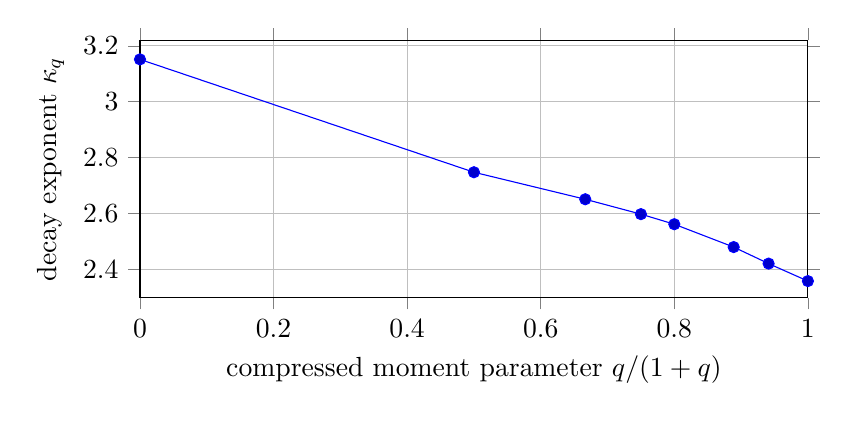
\begin{tikzpicture}
\begin{axis}[
 width=0.83\textwidth,height=0.40\textwidth,
 xlabel={compressed moment parameter \(q/(1+q)\)},
 ylabel={decay exponent \(\kappa_q\)},
 xmin=0,xmax=1,ymin=2.30,ymax=3.22,
 grid=major,tick align=outside]
\addplot+[mark=*] coordinates {
 (0,3.1514961295)
 (0.5,2.7480700149)
 (0.6666666667,2.6514961295)
 (0.75,2.5983138062)
 (0.8,2.5622414703)
 (0.8888888889,2.4805809434)
 (0.9411764706,2.4214870020)
 (1,2.3590148791)};
\end{axis}
\end{tikzpicture}
\end{center}

\section{The exact root-mean-square exponent}
\label{sec:rms}

The case \(q=2\) collapses to finite Fourier algebra; no numerical spectral computation is
needed.

\begin{theorem}[Exact quadratic lacunary identity]
\label{thm:exact-L2}
For every integer \(n\ge0\),
\begin{equation}
 \int_0^1\prod_{j=0}^{n-1}\sin^2(\pi2^jt)\dd t=2^{-n}.
 \label{eq:exact-L2}
\end{equation}
Equivalently, \(\rho_2=1/2\) and \(\Lambda_2=2^{-1/2}\).
\end{theorem}

\begin{proof}
By \Cref{prop:TM-polynomial},
\[
 P_n(t)=\sum_{k=0}^{2^n-1}\TM_k\e^{2\pi\ii kt},
 \qquad
 |P_n(t)|=2^n\prod_{j=0}^{n-1}|\sin(\pi2^jt)|.
\]
Parseval's identity for this finite Fourier polynomial gives
\[
 \int_0^1|P_n(t)|^2\dd t
 =\sum_{k=0}^{2^n-1}|\TM_k|^2=2^n.
\]
Dividing by \(4^n\) proves \eqref{eq:exact-L2}.

Alternatively, the transfer operator satisfies
\[
 \Transfer_2\mathbf1
 =\frac12\left(\sin^2\frac{\pi x}{2}+
                 \cos^2\frac{\pi x}{2}\right)=\frac12\mathbf1.
\]
Its positive leading eigenvalue is therefore \(1/2\), in agreement with the finite
identity.
\end{proof}

\begin{corollary}[RMS decay]
\label{cor:RMS}
The sharp root-mean-square exponent is
\begin{equation}
 \boxed{
 \kappa_2=\frac{\log(2\pi)}{\log2}}
 =2.651496129472318798\ldots .
 \label{eq:kappa2}
\end{equation}
There is \(A_2\in(0,\infty)\) such that
\begin{equation}
 \mathcal M_{2,n}\!\left(\frac{\PhiUp}{E_{\kappa_2}}\right)\longrightarrow A_2.
 \label{eq:RMS-limit}
\end{equation}
\end{corollary}

\begin{proof}
In \eqref{eq:kappa-from-Lambda}, insert \(\Lambda=2^{-1/2}\):
\[
 \kappa_2=\frac{\log\pi+a/2+a/2}{a}=\frac{\log(2\pi)}{a}.
\]
The convergence statement is the \(q=2\) case of \Cref{thm:Lq-spectrum}.
\end{proof}

\subsection{A discrete Parseval companion}

\begin{proposition}[Dyadic-grid identity]
\label{prop:grid-parseval}
For every \(n\ge1\), if
\(Q_n(t)=\prod_{j=0}^{n-1}|\sin(\pi2^jt)|\), then
\begin{equation}
 \sum_{m=0}^{2^n-1}Q_n(m/2^n)^2=1.
 \label{eq:grid-parseval}
\end{equation}
\end{proposition}

\begin{proof}
Let \(N=2^n\).  Discrete Parseval for the values of the degree-\((N-1)\) polynomial
\(P_n\) on the \(N\)th roots of unity gives
\[
 \sum_{m=0}^{N-1}|P_n(m/N)|^2
 =N\sum_{k=0}^{N-1}|\TM_k|^2=N^2.
\]
Since \(|P_n(t)|=NQ_n(t)\), division by \(N^2\) proves the claim.
\end{proof}

\subsection{Total Fourier energy and half-integer sampling}

\begin{proposition}[Energy sampling identity]
\label{prop:energy}
One has
\begin{equation}
 \int_{\R}|\PhiUp(x)|^2\dd x
 =\int_{\R}\up(t)^2\dd t
 =\frac12+\sum_{m=0}^{\infty}\PhiUp\!\left(m+\frac12\right)^2.
 \label{eq:energy}
\end{equation}
Numerically, the common value is
\(0.8088735359679705629\ldots\); this decimal is numerical evidence, not an interval
certificate.
\end{proposition}

\begin{proof}
The first equality is Plancherel's theorem under the convention
\eqref{eq:fourier-convention}.  Since \(\up\) is supported in \([-1,1]\), expand it as a
Fourier series of period two on that interval.  Its \(k\)th coefficient is
\[
 c_k=\frac12\int_{-1}^{1}\up(t)\e^{-\pi\ii kt}\dd t
 =\frac12\PhiUp(k/2).
\]
Parseval on an interval of length two gives
\[
 \int_{-1}^{1}\up(t)^2\dd t
 =2\sum_{k\in\Z}|c_k|^2
 =\frac12\sum_{k\in\Z}\PhiUp(k/2)^2.
\]
The \(k=0\) term contributes \(1/2\).  Every nonzero even \(k\) samples \(\PhiUp\) at a
nonzero integer and therefore vanishes by \Cref{prop:zeros}.  The positive and negative odd
terms pair by evenness.  Writing \(k=\pm(2m+1)\) yields \eqref{eq:energy}.
\end{proof}

\section{Arithmetic-mean decay and ordinary Ces\`aro averaging}
\label{sec:cesaro}

For \(q=1\), the transfer operator is
\begin{equation}
 (\Transfer_1f)(x)=\frac12\left[
 \sin\!\left(\frac{\pi x}{2}\right)f(x/2)
 +\cos\!\left(\frac{\pi x}{2}\right)f((x+1)/2)
 \right].
 \label{eq:L1}
\end{equation}
Its Perron root has no known elementary closed form, but it is a canonical spectral constant
and admits short exact enclosures.

\subsection{The Perron root and an exact rational certificate}

High-precision spectral computation gives
\begin{equation}
 \rho_1=0.661322602060565615\ldots,
 \qquad
 \boxed{
 \kappa_1=\frac{\log\pi+a/2-\log\rho_1}{a}}
 =2.748070014871332674\ldots .
 \label{eq:rho1-kappa1}
\end{equation}
The decimal is numerical.  The following enclosure, by contrast, is exact.

\begin{proposition}[Rational Collatz--Wielandt enclosure]
\label{prop:rho-certificate}
One has
\begin{equation}
 0.66126807<\rho_1<0.66134891,
 \label{eq:rho-bracket}
\end{equation}
and hence
\begin{equation}
 2.74801262<\kappa_1<2.74818899.
 \label{eq:kappa1-bracket}
\end{equation}
\end{proposition}

\begin{proof}
For any continuous \(f>0\), the eigenmeasure equation in
\eqref{eq:RPF-eigen} implies the Collatz--Wielandt bounds
\begin{equation}
 \min_{x\in[0,1]}\frac{\Transfer_1f(x)}{f(x)}
 \le\rho_1\le
 \max_{x\in[0,1]}\frac{\Transfer_1f(x)}{f(x)}.
 \label{eq:CW}
\end{equation}
Indeed, if \(mf\le\Transfer_1f\le Mf\), integration against \(\nu_1\) gives
\(m\nu_1(f)\le\rho_1\nu_1(f)\le M\nu_1(f)\), and \(\nu_1(f)>0\).

Choose
\begin{equation}
 p(u)=1+\frac{376189}{10^6}u-\frac{69093}{10^6}u^2
       +\frac{15483}{10^6}u^3,
 \qquad f(x)=p(\sin\pi x).
 \label{eq:certificate-p}
\end{equation}
The polynomial is positive on \([0,1]\), since
\(p(u)\ge1-69093/10^6>0\).  Put
\[
 t=\tan\frac{\pi x}{4},\qquad
 u=\sin\frac{\pi x}{2}=\frac{2t}{1+t^2},\qquad
 v=\cos\frac{\pi x}{2}=\frac{1-t^2}{1+t^2}.
\]
As \(x\) runs from zero to one, \(t\) runs from zero to one, and
\(\sin\pi x=2uv\).  Therefore
\begin{equation}
 \frac{\Transfer_1f(x)}{f(x)}
 =R(t)\defeq\frac{u\,p(u)+v\,p(v)}{2p(2uv)},
 \qquad 0\le t\le1.
 \label{eq:R-certificate}
\end{equation}
After clearing the positive denominator, the inequalities
\[
 \frac{66126807}{10^8}<R(t)<\frac{66134891}{10^8}
\]
become positivity of two explicit integer polynomials of degree twelve.  Their Sturm chains
have the same number of sign variations at \(0\) and \(1\), namely six, and both
polynomials are positive at zero.  Hence neither has a root on \([0,1]\), and both remain
positive there.  The complete exact integer computation is reproduced in
\Cref{app:certificate}; no floating-point step enters this sign proof.  Applying
\eqref{eq:CW} gives \eqref{eq:rho-bracket}.  Formula \eqref{eq:kappa1-bracket} follows from
the strictly decreasing map
\(r\mapsto(\log\pi+a/2-\log r)/a\).
\end{proof}

\begin{remark}
Aistleitner--Hofer--Larcher \cite{ahl} give the sharper rigorous interval
\(0.66130<\rho_1<0.66135\) by a transfer recursion.  The slightly wider bracket above is
retained because it can be checked from one small polynomial and exact Sturm arithmetic.
\end{remark}

\subsection{The natural arithmetic-mean gauge}

By \Cref{thm:Lq-spectrum},
\begin{equation}
 2\int_{1/2}^{1}
 \frac{\abs{\PhiUp(2^ny)}}{E_{\kappa_1}(2^ny)}\dd y
 \longrightarrow A_1,
 \label{eq:A1-limit}
\end{equation}
where the exact spectral expression is
\begin{equation}
 A_1=\left(\int_0^1h_1(x)\dd x\right)
 \nu_1\!\left(W_{\kappa_1}((\,\cdot\,+1)/2)\right).
 \label{eq:A1-exact}
\end{equation}
Numerically,
\begin{equation}
 A_1=0.091266124131588\ldots .
 \label{eq:A1-numeric}
\end{equation}
Define
\begin{equation}
 g_1(x)=A_1E_{\kappa_1}(x).
 \label{eq:g1}
\end{equation}
Then the mean of \(\abs{\PhiUp}/g_1\) on every complete dyadic shell tends to one.

\begin{proposition}[Regularity of the natural gauge]
\label{prop:g1-regularity}
The gauge \(g_1\) is positive and real analytic on \((0,\infty)\), and it is strictly
decreasing for \(x\ge1\).  For every fixed integer \(m\ge0\), there is \(X_m\) such that
\begin{equation}
 (-1)^mg_1^{(m)}(x)>0,
 \qquad x\ge X_m.
 \label{eq:alternating-derivatives}
\end{equation}
\end{proposition}

\begin{proof}
Put \(u=\log x\) and
\[
 G(u)=g_1(\e^u)=A_1\exp\!\left(-\frac{u^2}{2a}-\kappa_1u\right).
\]
Analyticity and positivity are immediate.  Directly,
\[
 \frac{g_1'(x)}{g_1(x)}=-\frac{u/a+\kappa_1}{x}<0
\]
for \(x\ge1\).  For higher derivatives use
\[
 x^m\frac{\dd^m}{\dd x^m}
 =D_u(D_u-1)\cdots(D_u-m+1),
 \qquad D_u=\frac{\dd}{\dd u}.
\]
Let \(P(u)=u/a+\kappa_1\).  Since \(D_uG=-P(u)G\), induction on \(m\) gives
\begin{equation}
 (-1)^m\frac{x^mg_1^{(m)}(x)}{g_1(x)}
 =P(u)^m+O_m(P(u)^{m-1}).
 \label{eq:derivative-asymptotic}
\end{equation}
The leading term is positive and dominates as \(u\to\infty\), proving
\eqref{eq:alternating-derivatives}.
\end{proof}

\begin{corollary}[Dyadic Ces\`aro convergence and unrestricted boundedness]
\label{cor:dyadic-Cesaro}
For every fixed \(t_0>0\),
\begin{equation}
 \frac1{2^n-t_0}\int_{t_0}^{2^n}
 \frac{\abs{\PhiUp(x)}}{g_1(x)}\dd x\longrightarrow1.
 \label{eq:dyadic-Cesaro}
\end{equation}
Moreover,
\begin{equation}
 0<\liminf_{t\to\infty}\frac1{t-t_0}\int_{t_0}^{t}
 \frac{\abs{\PhiUp(x)}}{g_1(x)}\dd x
 \le
 \limsup_{t\to\infty}\frac1{t-t_0}\int_{t_0}^{t}
 \frac{\abs{\PhiUp(x)}}{g_1(x)}\dd x<\infty.
 \label{eq:Cesaro-bounded}
\end{equation}
\end{corollary}

\begin{proof}
Let
\[
 a_n=\frac1{2^{n-1}}\int_{2^{n-1}}^{2^n}
 \frac{\abs{\PhiUp(x)}}{g_1(x)}\dd x.
\]
Equation \eqref{eq:A1-limit} says \(a_n\to1\).  Therefore
\[
 \int_{1}^{2^N}\frac{\abs{\PhiUp(x)}}{g_1(x)}\dd x
 =\sum_{n=1}^{N}2^{n-1}a_n.
\]
A weighted Ces\`aro argument gives
\(
 2^{-N}\sum_{n=1}^{N}2^{n-1}a_n\to1
\): split the sum at a fixed index after which \(|a_n-1|<\varepsilon\), and note that the
finite initial part is \(o(2^N)\).  This proves \eqref{eq:dyadic-Cesaro}; changing the fixed
lower endpoint contributes only \(O(1)/2^N\).

If \(2^{N-1}\le t\le2^N\), the completed shells up to \(2^{N-1}\) give a lower bound
asymptotic to \(2^{N-1}\), while including the entire current shell gives an upper bound
asymptotic to \(2^N\).  Since \(t\) lies between those same quantities, division by \(t\)
gives positive finite uniform lower and upper bounds.  Again, a fixed \(t_0\) is negligible.
\end{proof}

\subsection{The endpoint phase left by an incomplete shell}

The previous corollary does \emph{not} imply an unrestricted limit.  A final incomplete
shell contributes a fixed fraction of the total additive average, and its normalized mass
converges to a singular distribution.

Let
\begin{equation}
 f_1(x)=W_{\kappa_1}\!\left(\frac{x+1}{2}\right),
 \qquad
 D(z)=\frac{\nu_1(f_1\ind_{[0,z]})}{\nu_1(f_1)},
 \qquad 0\le z\le1.
 \label{eq:D-def}
\end{equation}

\begin{lemma}[The limiting shell measure is continuous and singular]
\label{lem:singular-measure}
The probability measure
\begin{equation}
 \mu(A)=\frac{\nu_1(f_1\ind_A)}{\nu_1(f_1)}
 \label{eq:mu-def}
\end{equation}
is atomless, fully supported, and singular with respect to Lebesgue measure.  Consequently
\(D\) is a continuous, nondecreasing singular distribution function with
\(D(0)=0\) and \(D(1)=1\).
\end{lemma}

\begin{proof}
Primitivity in the proof of \Cref{prop:RPF} implies that \(\nu_1\) gives positive mass to
every nonempty open interval.  Since \(f_1\) is continuous and positive on \([0,1)\), the
same is true for \(\mu\).

We next rule out atoms.  The transfer weights at the endpoints show directly from
\(\Transfer_1^*\nu_1=\rho_1\nu_1\) that \(\nu_1(\{0\})=\nu_1(\{1\})=0\).  The possible
atom at \(1/2\) is fed only by these endpoint atoms and also vanishes.  At any other
\(z\in(0,1)\), testing the eigenmeasure equation on a shrinking neighborhood of \(z\)
gives
\begin{equation}
 \rho_1\nu_1(\{z\})=\frac12s(z)\nu_1(\{Tz\}).
 \label{eq:atom-propagation}
\end{equation}
If \(\nu_1(\{z\})>0\), then
\(
 \nu_1(\{Tz\})\ge2\rho_1\nu_1(\{z\})
\), and \(2\rho_1>1\) by \eqref{eq:rho-bracket}.  A periodic forward orbit gives a
contradiction after one cycle; a nonperiodic orbit produces infinitely many distinct atoms
whose masses grow geometrically, contradicting finiteness.  Thus \(\nu_1\), and hence
\(\mu\), is atomless.

Finally suppose \(\nu_1\) had a nonzero absolutely continuous part \(r(x)\dd x\).  Weighted
composition by Lipschitz branches preserves the Lebesgue decomposition, so this part must
itself satisfy the eigenmeasure equation.  A change of variables in
\(
 \int\Transfer_1\varphi\,r\dd x=\rho_1\int\varphi r\dd x
\)
gives
\begin{equation}
 \rho_1r(x)=s(x)r(Tx)
 \quad\text{for almost every }x.
 \label{eq:conformal-density}
\end{equation}
On the set where \(r(x)>0\), iteration yields
\begin{equation}
 r(T^nx)=r(x)\frac{\rho_1^n}
 {\prod_{j=0}^{n-1}s(T^jx)}.
 \label{eq:density-iterate}
\end{equation}
For Lebesgue-almost every \(x\), Birkhoff's theorem makes the logarithmic growth rate of the
right side \(\log(2\rho_1)>0\).  On the other hand, for every \(\varepsilon>0\), invariance
of Lebesgue measure and Markov's inequality give
\[
 \sum_{n=1}^{\infty}
 \Leb\{x:r(T^nx)>\e^{\varepsilon n}\}
 =\sum_{n=1}^{\infty}\Leb\{r>\e^{\varepsilon n}\}
 \le\norm{r}_1\sum_{n=1}^{\infty}\e^{-\varepsilon n}<\infty.
\]
Borel--Cantelli implies \(r(T^nx)\le e^{\varepsilon n}\) eventually for almost every
\(x\).  Choosing \(\varepsilon<\log(2\rho_1)\) contradicts
\eqref{eq:density-iterate} wherever \(r(x)>0\).  Hence the absolutely continuous part is
zero and \(\nu_1\) is singular.  Multiplication by the continuous function \(f_1\) preserves
singularity.
\end{proof}

\begin{theorem}[Exact dyadic phase profile]
\label{thm:phase-profile}
For every \(y\in[1/2,1]\) and every fixed \(t_0>0\),
\begin{equation}
 \lim_{n\to\infty}
 \frac1{2^ny-t_0}\int_{t_0}^{2^ny}
 \frac{\abs{\PhiUp(x)}}{g_1(x)}\dd x
 =P(y)\defeq\frac{1+D(2y-1)}{2y}.
 \label{eq:phase-profile}
\end{equation}
The function \(P\) is continuous, satisfies \(P(1/2)=P(1)=1\), and is not constant.
Therefore the unrestricted ordinary Ces\`aro limit for the natural gauge \(g_1\) does not
exist.
\end{theorem}

\begin{proof}
The spectral decomposition \eqref{eq:RPF-gap}, first for H\"older test functions and then
by upper and lower H\"older approximation of \(\ind_{[0,z]}\), gives
\begin{equation}
 \rho_1^{-n}\int_0^z f_1(x)
 \prod_{j=0}^{n-1}s(T^jx)\dd x
 \longrightarrow
 \left(\int_0^1h_1\right)\nu_1(f_1\ind_{[0,z]}).
 \label{eq:partial-RPF}
\end{equation}
The squeezing step is valid because \(\nu_1\) has no atoms.  Returning through
\(x=2y-1\), the partial integral over the current shell satisfies
\begin{equation}
 \int_{2^{n-1}}^{2^ny}\frac{\abs{\PhiUp(x)}}{g_1(x)}\dd x
 =2^{n-1}D(2y-1)+o(2^n).
 \label{eq:partial-shell}
\end{equation}
The sum of all preceding complete shells is
\(2^{n-1}+o(2^n)\) by \Cref{cor:dyadic-Cesaro}.  Dividing the sum of these two contributions
by \(2^ny\) proves \eqref{eq:phase-profile}; a fixed lower endpoint is negligible.

The endpoint values follow from \(D(0)=0\) and \(D(1)=1\).  If \(P\equiv1\), then
\(1+D(2y-1)=2y\), so after putting \(z=2y-1\) one obtains \(D(z)=z\).  That would make
\(\mu\) Lebesgue measure, contradicting the singularity in
\Cref{lem:singular-measure}.
\end{proof}

\begin{center}
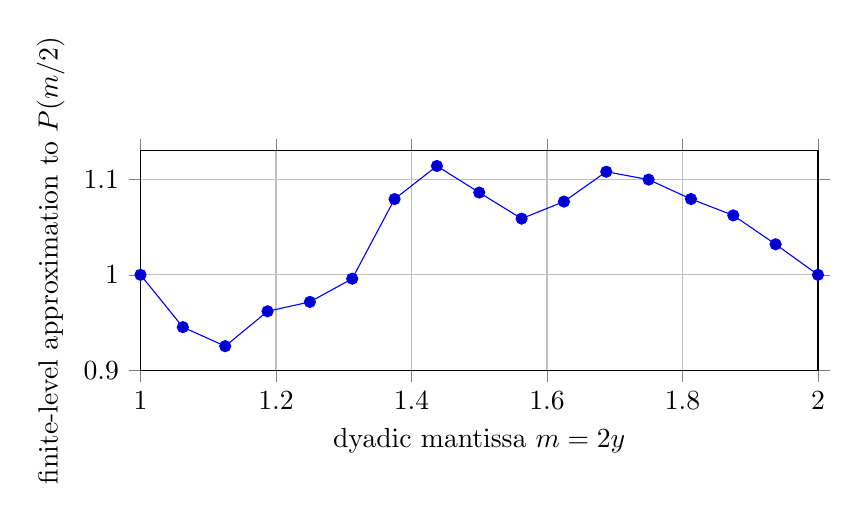
\begin{tikzpicture}
\begin{axis}[
 width=0.84\textwidth,height=0.36\textwidth,
 xlabel={dyadic mantissa \(m=2y\)},ylabel={finite-level approximation to \(P(m/2)\)},
 xmin=1,xmax=2,ymin=0.90,ymax=1.13,grid=major,tick align=outside]
\addplot+[mark=*] coordinates {
 (1.0000,1.000000000) (1.0625,0.945118496) (1.1250,0.925107303)
 (1.1875,0.961711083) (1.2500,0.971580861) (1.3125,0.995925058)
 (1.3750,1.079490550) (1.4375,1.114228254) (1.5000,1.086316716)
 (1.5625,1.058951765) (1.6250,1.076832568) (1.6875,1.108201849)
 (1.7500,1.099910476) (1.8125,1.079553278) (1.8750,1.062385735)
 (1.9375,1.032028829) (2.0000,1.000000000)};
\end{axis}
\end{tikzpicture}
\end{center}

\begin{meaningbox}
Complete shells are normalized correctly, but an additive average gives the last incomplete
shell macroscopic weight.  Its mass does not become uniform: it converges to the singular
conformal measure \(\mu\).  This is why a power of \(\log x\), or any other slowly varying
scalar correction, cannot remove the endpoint dependence.
\end{meaningbox}

\section{How strong is the Ces\`aro obstruction?}
\label{sec:obstruction}

The failure in \Cref{thm:phase-profile} is not caused merely by choosing the wrong constant.
It survives every correction whose variation inside one dyadic shell remains bounded after
an arbitrary shellwise rescaling.

On the shell \([2^k,2^{k+1}]\), use the coordinate \(x=2^k(1+z)\), \(0\le z\le1\), and
define the finite measure
\begin{equation}
 \dd\mu_k(z)=D_k(z)\dd z,
 \qquad
 D_k(z)=\frac{\abs{\PhiUp(2^k(1+z))}}{g_1(2^k(1+z))}.
 \label{eq:mu-k}
\end{equation}
The transfer-operator limit gives
\begin{equation}
 \mu_k\Longrightarrow\mu,
 \qquad \mu_k([0,1])\longrightarrow1,
 \label{eq:mu-k-limit}
\end{equation}
where \(\mu\) is the singular probability measure in \Cref{lem:singular-measure}.

\begin{theorem}[Bounded-distortion obstruction]
\label{thm:bounded-distortion}
Let \(g:[X_0,\infty)\to(0,\infty)\) be measurable.  Suppose there are constants
\(0<m<M<\infty\) and positive shell scalars \(c_k\) such that, for all sufficiently large
\(k\) and every \(z\in[0,1]\),
\begin{equation}
 m\le\frac{g(2^k(1+z))}{c_kg_1(2^k(1+z))}\le M.
 \label{eq:bounded-distortion}
\end{equation}
Then \(g\) cannot satisfy
\begin{equation}
 \frac1{t-X_0}\int_{X_0}^{t}\frac{\abs{\PhiUp(x)}}{g(x)}\dd x\longrightarrow1.
 \label{eq:unrestricted-target}
\end{equation}
\end{theorem}

\begin{proof}
Assume \eqref{eq:unrestricted-target}.  Write its numerator as \(I(t)\).  For every fixed
\(0\le z_1<z_2\le1\), subtract the asymptotics at the two endpoints
\(2^k(1+z_i)\).  Since \(I(t)=t-X_0+o(t)\),
\begin{equation}
 \frac{I(2^k(1+z_2))-I(2^k(1+z_1))}{2^k}
 \longrightarrow z_2-z_1.
 \label{eq:shell-linearity}
\end{equation}
In particular, after normalization by its total mass, the measure induced by
\(\abs{\PhiUp}/g\) on the \(k\)th shell must converge weakly to Lebesgue measure on
\([0,1]\).

Remove the irrelevant scalar \(c_k\) by putting
\[
 q_k(z)=\frac{c_kg_1(2^k(1+z))}{g(2^k(1+z))}.
\]
Then \(M^{-1}\le q_k\le m^{-1}\), and the normalized shell probability measure is
\begin{equation}
 \dd\eta_k(z)=
 \frac{q_k(z)\dd\mu_k(z)}{\int_0^1q_k\dd\mu_k}.
 \label{eq:eta-k}
\end{equation}
Let \(a_k=\mu_k([0,1])\) and \(\bar\mu_k=a_k^{-1}\mu_k\).  Because
\(\int q_k\dd\mu_k\ge a_k/M\), for every continuous \(\varphi\ge0\),
\begin{equation}
 \int\varphi\dd\eta_k
 \le\frac{M}{m}\int\varphi\dd\bar\mu_k.
 \label{eq:measure-domination}
\end{equation}
Take a weakly convergent subsequence of \(\eta_k\).  Equation
\eqref{eq:mu-k-limit} and \eqref{eq:measure-domination} imply that its limit \(\eta\) is
dominated by \((M/m)\mu\).  Hence \(\eta\) is singular.  But
\eqref{eq:shell-linearity} forces the entire sequence \(\eta_k\) to converge to Lebesgue
measure, a contradiction.
\end{proof}

\begin{corollary}[Necessary shell microstructure]
\label{cor:microstructure}
Every gauge satisfying \eqref{eq:unrestricted-target} must have unbounded within-shell
distortion relative to \(g_1\), even after arbitrary scalar rescaling on each shell.
In particular, the following corrections cannot work:
\begin{enumerate}
\item powers or iterated powers of \(\log x\);
\item regularly varying multipliers;
\item fixed continuous log-periodic factors;
\item any positive oscillatory multiplier bounded above and bounded away from zero.
\end{enumerate}
\end{corollary}

\begin{proof}
Each listed class satisfies \eqref{eq:bounded-distortion} for suitable shell scalars.  For a
slowly varying multiplier \(L\), the uniform convergence theorem gives
\(L(2^k(1+z))/L(2^k)\to1\) uniformly in \(z\in[0,1]\).  Fixed log-periodic or bounded
oscillatory multipliers are bounded above and below.  The conclusion follows from
\Cref{thm:bounded-distortion}.
\end{proof}

\begin{pitfallbox}
The theorem does not say that no analytic or no ``explicit-looking'' gauge can work.  It
says that a successful gauge must develop increasingly fine and increasingly large relative
variation inside successive dyadic shells.  That observation points directly to the
adaptive construction in the next section.
\end{pitfallbox}

\section{A shell-adaptive analytic gauge with an exact limit}
\label{sec:adaptive}

The singular shell measure can be flattened at each finite level.  By increasing the
resolution slowly enough, the flattening multipliers have logarithms and logarithmic slopes
of size \(o(k)\) on the \(k\)th shell.  The baseline \(1/g_1\) has slope of order \(k\), so
the resulting reciprocal gauge remains increasing, and the gauge itself remains decreasing.

\subsection{A quantitative smooth-flattening lemma}

\begin{lemma}[Smooth flattening of weakly convergent measures]
\label{lem:flattening}
Let \(\sigma_k\) be finite positive Borel measures on \([0,1]\) such that
\(
 \sigma_k\Rightarrow\sigma
\) and \(\sigma_k([0,1])\to1\), where \(\sigma\) is an atomless, fully supported
probability measure.  Then there are positive functions \(r_k\in C^\infty[0,1]\) with the
following properties:
\begin{enumerate}
\item \(r_k\equiv1\) on neighborhoods of both endpoints;
\item the weighted cumulative masses become uniformly linear:
\begin{equation}
 \sup_{0\le z\le1}
 \left|\int_0^zr_k\dd\sigma_k-z\right|\longrightarrow0;
 \label{eq:flattening-CDF}
\end{equation}
\item the flattening changes slowly compared with the shell index:
\begin{equation}
 \norm{\log r_k}_\infty=o(k),
 \qquad
 \norm{(\log r_k)'}_\infty=o(k).
 \label{eq:flattening-bounds}
\end{equation}
\end{enumerate}
\end{lemma}

\begin{proof}
We separate finite-resolution equalization from a diagonal choice of resolution.

\emph{Step 1: choose finite partitions.}
For each \(j\ge1\), choose a partition
\[
 0=x_{j,0}<x_{j,1}<\cdots<x_{j,N_j}=1
\]
with mesh at most \(\varepsilon_j\), where \(\varepsilon_j\downarrow0\).  Because \(\sigma\)
is atomless, all boundary points are continuity points.  Because \(\sigma\) has full
support, every cell \(I_{j,i}=[x_{j,i-1},x_{j,i}]\) has positive \(\sigma\)-mass.
For fixed \(j\), weak convergence gives simultaneous convergence
\(
 \sigma_k(I_{j,i})\to\sigma(I_{j,i})
\) over the finitely many cells.  Hence, for large \(k\), the cell equalizers
\begin{equation}
 c_{k,j,i}=\frac{|I_{j,i}|}{\sigma_k(I_{j,i})}
 \label{eq:cell-equalizer}
\end{equation}
are positive and bounded above and below by constants depending only on \(j\).  Choose
\(B_j\) so that \(|\log c_{k,j,i}|\le B_j/2\) for all these cells and all sufficiently
large \(k\).

\emph{Step 2: smooth the jumps on a negligible set.}
Choose a finite union \(U_j\) of small intervals around all partition boundaries, including
the endpoints, so that \(\sigma(\partial U_j)=0\) and
\begin{equation}
 \sigma(U_j)+|U_j|<\frac{\varepsilon_j\e^{-B_j}}{20}.
 \label{eq:small-transition-set}
\end{equation}
Weak convergence gives \(\sigma_k(U_j)\to\sigma(U_j)\).  Outside \(U_j\), set
\(\ell_{k,j}=\log c_{k,j,i}\) on the interior of each cell.  Inside \(U_j\), join adjacent
constant values smoothly, without leaving their convex hull, and arrange
\(\ell_{k,j}=0\) near \(0\) and \(1\).  Since there are only finitely many transitions for
fixed \(j\), the interpolation may be chosen with
\begin{equation}
 \norm{\ell_{k,j}}_\infty\le B_j,
 \qquad
 \norm{\ell_{k,j}'}_\infty\le C_j
 \label{eq:ell-bounds}
\end{equation}
for some \(C_j<\infty\) independent of sufficiently large \(k\).  Put
\(r_{k,j}=\exp\ell_{k,j}\).

On a complete cell \(I=I_{j,i}\), the exact equality
\(c_{k,j,i}\sigma_k(I)=|I|\) implies
\begin{equation}
 \int_Ir_{k,j}\dd\sigma_k-|I|
 =\int_{I\cap U_j}(r_{k,j}-c_{k,j,i})\dd\sigma_k.
 \label{eq:cell-error}
\end{equation}
The total error over any union of complete cells is therefore at most
\(2\e^{B_j}\sigma_k(U_j)\).  A cumulative interval \([0,z]\) contains at most one partial
cell.  Away from \(U_j\), the weighted mass of that partial cell is at most its full length,
and inside \(U_j\) it is at most \(e^{B_j}\sigma_k(U_j)\).  The missing Lebesgue length is
bounded by the mesh and \(|U_j|\).  By \eqref{eq:small-transition-set}, for all sufficiently
large \(k\),
\begin{equation}
 \sup_z\left|\int_0^zr_{k,j}\dd\sigma_k-z\right|\le3\varepsilon_j.
 \label{eq:finite-resolution-error}
\end{equation}

\emph{Step 3: let the resolution increase diagonally.}
Choose integers \(K_j\uparrow\infty\) so large that all preceding estimates hold for
\(k\ge K_j\) and, in addition,
\begin{equation}
 \frac{B_j}{K_j}\le\varepsilon_j,
 \qquad
 \frac{C_j}{K_j}\le\varepsilon_j.
 \label{eq:diagonal-budget}
\end{equation}
For \(K_j\le k<K_{j+1}\), set \(r_k=r_{k,j}\).  Then \(j=j(k)\to\infty\), so
\eqref{eq:finite-resolution-error} proves \eqref{eq:flattening-CDF};
\eqref{eq:ell-bounds} and \eqref{eq:diagonal-budget} prove
\eqref{eq:flattening-bounds}.  The endpoint condition was built into the smoothing.
\end{proof}

\subsection{The smooth adaptive gauge}

Apply \Cref{lem:flattening} to \(\sigma_k=\mu_k\) and \(\sigma=\mu\).  On each sufficiently
large shell define
\begin{equation}
 R(2^k(1+z))=r_k(z),
 \qquad 0\le z\le1.
 \label{eq:R-global}
\end{equation}
Because \(r_k=1\) near both endpoints, adjacent shell definitions agree with all derivatives
near powers of two.  Thus \(R\) is \(C^\infty\) on a half-line.  Put
\begin{equation}
 h_0(x)=\frac1{g_1(x)},
 \qquad h(x)=h_0(x)R(x),
 \qquad g_\infty(x)=\frac1{h(x)}.
 \label{eq:smooth-adaptive}
\end{equation}

\begin{lemma}[The adaptive gauge remains decreasing]
\label{lem:adaptive-monotone}
For all sufficiently large \(x\), \(h'(x)>0\) and \(g_\infty'(x)<0\).  Moreover,
\begin{equation}
 \log g_\infty(x)=\log g_1(x)+o(\log x).
 \label{eq:adaptive-rough-smooth}
\end{equation}
\end{lemma}

\begin{proof}
In the shell coordinate \(x=2^k(1+z)\), direct differentiation gives
\begin{equation}
 \frac{\partial}{\partial z}\log h_0(2^k(1+z))
 =\frac{k+\kappa_1+a^{-1}\log(1+z)}{1+z}.
 \label{eq:baseline-slope}
\end{equation}
Uniformly in \(z\in[0,1]\), this is at least \(k/3\) for large \(k\).  On the other hand,
\(
 \partial_z\log R=(\log r_k)'
\) has supremum norm \(o(k)\) by \eqref{eq:flattening-bounds}.  Therefore
\(\partial_z\log h>0\) eventually.  Since \(z\) increases with \(x\), \(h'>0\) and
\(g_\infty'=-(h'/h^2)<0\).

Also \(\log g_\infty=\log g_1-\log R\).  On the \(k\)th shell,
\(\norm{\log R}_\infty=o(k)\), while \(k\asymp\log x\), proving
\eqref{eq:adaptive-rough-smooth}.
\end{proof}

\begin{proposition}[Smooth exact arithmetic gauge]
\label{prop:smooth-adaptive}
After an arbitrary positive smooth extension over an initial compact interval, the gauge
\(g_\infty\) satisfies, for every fixed \(X_0>0\),
\begin{equation}
 \frac1{t-X_0}\int_{X_0}^{t}
 \frac{\abs{\PhiUp(x)}}{g_\infty(x)}\dd x\longrightarrow1.
 \label{eq:smooth-exact-limit}
\end{equation}
\end{proposition}

\begin{proof}
Define
\[
 C_k(z)=\int_0^zD_k(u)r_k(u)\dd u.
\]
By \Cref{lem:flattening},
\(
 \varepsilon_k\defeq\sup_z|C_k(z)-z|\to0
\).  If \(t=2^K(1+z)\), complete and partial shells give, up to one fixed initial
contribution,
\begin{equation}
 \int_{X_0}^{t}\frac{\abs{\PhiUp(x)}}{g_\infty(x)}\dd x
 =\sum_{k<K}2^kC_k(1)+2^KC_K(z).
 \label{eq:adaptive-shell-sum}
\end{equation}
Replacing \(C_k(1)\) by one and \(C_K(z)\) by \(z\) costs
\[
 O(1)+\sum_{k<K}2^k\varepsilon_k+2^K\varepsilon_K=o(2^K).
\]
Indeed, for any \(\varepsilon>0\), all sufficiently late \(\varepsilon_k\) are below
\(\varepsilon\), while the finitely many earlier terms are \(o(2^K)\).  The main term is
\[
 \sum_{k<K}2^k+2^Kz=t+O(1),
\]
after the fixed initial shells are absorbed into the constant.  Division by \(t-X_0\)
proves \eqref{eq:smooth-exact-limit}.
\end{proof}

\subsection{Real-analytic upgrade}

We use Hoischen's derivative form of Carleman approximation: if
\(f\in C^1(\R)\) and \(\epsilon:\R\to(0,\infty)\) is continuous, there is an entire
function \(F\), real on \(\R\), such that
\begin{equation}
 |F(x)-f(x)|<\epsilon(x),
 \qquad |F'(x)-f'(x)|<\epsilon(x)
 \quad(x\in\R).
 \label{eq:Hoischen}
\end{equation}
See Gauthier--Kienzle \cite{gauthier-kienzle} for a convenient modern formulation.

\begin{theorem}[Positive analytic adaptive gauge]
\label{thm:analytic-adaptive}
There exists a positive real-analytic strictly decreasing function
\(g_{\mathrm{ad}}:(0,\infty)\to(0,\infty)\) such that, for every fixed \(t_0>0\),
\begin{equation}
 \frac1{t-t_0}\int_{t_0}^{t}
 \frac{\abs{\PhiUp(x)}}{g_{\mathrm{ad}}(x)}\dd x\longrightarrow1,
 \label{eq:analytic-adaptive-limit}
\end{equation}
and
\begin{equation}
 \log g_{\mathrm{ad}}(x)
 =-\frac{(\log x)^2}{2\log2}-\kappa_1\log x+o(\log x).
 \label{eq:analytic-adaptive-scale}
\end{equation}
\end{theorem}

\begin{proof}
Extend the function \(h=1/g_\infty\) from a sufficiently far tail to a positive
\(C^1\) function on \(\R\) with \(h'(x)>0\) everywhere.  This can be done on the remaining
compact interval by monotone Hermite interpolation, or by joining to a positive exponential.
Choose any continuous \(\delta(x)>0\) with \(\delta(x)\to0\) as \(x\to+\infty\), and then
a continuous positive tolerance satisfying
\begin{equation}
 \epsilon(x)<\frac12\min\{h(x),h'(x),\delta(x)h(x)\}.
 \label{eq:analytic-tolerance}
\end{equation}
Apply \eqref{eq:Hoischen}.  The resulting real entire function \(\widetilde h\) obeys
\(
 \widetilde h>h/2>0
\) and \(\widetilde h'>h'/2>0\) on \(\R\), and
\begin{equation}
 \frac{\widetilde h(x)}{h(x)}\longrightarrow1.
 \label{eq:h-relative}
\end{equation}
Define \(g_{\mathrm{ad}}=1/\widetilde h\) on \((0,\infty)\).  It is positive, real analytic,
and strictly decreasing.

Equation \eqref{eq:h-relative}, together with
\eqref{eq:adaptive-rough-smooth}, proves the logarithmic scale
\eqref{eq:analytic-adaptive-scale}.  To preserve the average, fix \(\varepsilon>0\) and
choose \(X\) so that \(|\widetilde h/h-1|<\varepsilon\) for \(x\ge X\).  Then
\begin{align*}
 \left|\int_X^t\abs{\PhiUp(x)}(\widetilde h(x)-h(x))\dd x\right|
 &\le\varepsilon\int_X^t\abs{\PhiUp(x)}h(x)\dd x\\
 &=\varepsilon(t+o(t))
\end{align*}
by \Cref{prop:smooth-adaptive}.  The compact initial interval contributes \(O(1)\).
Divide by \(t\), let \(t\to\infty\), and then let \(\varepsilon\downarrow0\).  This proves
\eqref{eq:analytic-adaptive-limit}.
\end{proof}

\begin{remark}
There is no contradiction with \Cref{thm:bounded-distortion}.  At level \(k\), the
flattening corrects only a finite partition, but the number of cells tends to infinity.  Its
logarithm and logarithmic slope are \(o(k)\), so monotonicity survives, while its distortion
relative to \(g_1\) becomes unbounded and its shell shape never stabilizes.
\end{remark}

\section{The multiplicatively natural logarithmic mean}
\label{sec:logmean}

The endpoint phase is specific to additive averaging.  Under \(\dd x/x\), every complete
dyadic shell has the same weight \(\log2\), and one incomplete shell is negligible among
\(N\) completed shells.

\begin{theorem}[Unrestricted logarithmic mean]
\label{thm:logarithmic-mean}
For every fixed \(t_0>1\),
\begin{equation}
 \frac1{\log(t/t_0)}\int_{t_0}^{t}
 \frac{\abs{\PhiUp(x)}}{E_{\kappa_1}(x)}\frac{\dd x}{x}
 \longrightarrow A_1^{\log},
 \label{eq:logarithmic-mean}
\end{equation}
where
\begin{equation}
 A_1^{\log}
 =\frac1{\log2}\left(\int_0^1h_1(x)\dd x\right)
 \nu_1\!\left(\frac{f_1}{1+\,\cdot\,}\right)>0.
 \label{eq:A1log}
\end{equation}
Numerically,
\begin{equation}
 A_1^{\log}=0.09386063575678126354\ldots .
 \label{eq:A1log-num}
\end{equation}
\end{theorem}

\begin{proof}
For the shell \([2^{n-1},2^n]\), put
\[
 \beta_n=\int_{2^{n-1}}^{2^n}
 \frac{\abs{\PhiUp(x)}}{E_{\kappa_1}(x)}\frac{\dd x}{x}.
\]
Use \(x=2^ny\), then \(z=2y-1\).  Since \(\dd x/x=\dd z/(1+z)\), the master
factorization gives
\begin{equation}
 \beta_n=\rho_1^{-n}\int_0^1
 \frac{f_1(z)}{1+z}\prod_{j=0}^{n-1}s(T^jz)\dd z.
 \label{eq:beta-n}
\end{equation}
The RPF limit implies
\[
 \beta_n\longrightarrow
 B_1\defeq\left(\int_0^1h_1\right)
 \nu_1\!\left(\frac{f_1}{1+\,\cdot\,}\right).
\]
If \(2^N\le t<2^{N+1}\), the logarithmic numerator is the sum of \(N+O(1)\) complete-shell
terms \(\beta_n\), plus one partial-shell term.  The latter is uniformly bounded because it
is bounded by the full positive shell integral.  Hence the numerator is
\(NB_1+o(N)\), while \(\log(t/t_0)=Na+O(1)\).  Their quotient tends to \(B_1/a\), which is
\eqref{eq:A1log}.
\end{proof}

\section{The sharp uniform envelope}
\label{sec:uniform}

The preceding norms describe the bulk of a dyadic shell.  We now ask for the largest
possible numerator.  This is an ergodic-optimization problem, but in the dyadic case its
sharp exponential rate follows from one elementary two-step inequality.

Put
\begin{equation}
 \lambda\defeq\frac{\sqrt3}{2},
 \qquad \beta\defeq\log\lambda<0.
 \label{eq:lambda-beta}
\end{equation}

\begin{lemma}[Sharp two-step sine inequality]
\label{lem:sharp-sine-inequality}
For every real \(x\),
\begin{equation}
 \frac23\log s(x)+\frac13\log s(Tx)\le\log\lambda,
 \label{eq:weighted-log-sine}
\end{equation}
where the left-hand side is interpreted as \(-\infty\) if one of the factors vanishes.
Equality holds precisely when
\(x\equiv1/3\) or \(2/3\pmod1\).
\end{lemma}

\begin{proof}
Since all factors are nonnegative, exponentiating three times shows that
\eqref{eq:weighted-log-sine} is equivalent to
\begin{equation}
 s(x)^2s(Tx)\le\lambda^3.
 \label{eq:cubed-sine-ineq}
\end{equation}
Let \(\theta=\pi x\) and \(u=\sin^2\theta\).  Because
\(s(Tx)=|\sin(2\theta)|=2|\sin\theta\cos\theta|\),
\[
 s(x)^2s(Tx)=2|\sin^3\theta\cos\theta|.
\]
Squaring reduces the maximization to
\[
 4u^3(1-u),\qquad 0\le u\le1.
\]
Its derivative is \(4u^2(3-4u)\); hence its unique interior maximum is attained at
\(u=3/4\), and the maximum value is \(27/64\).  Taking square roots gives
\[
 s(x)^2s(Tx)\le\frac{3\sqrt3}{8}
 =\left(\frac{\sqrt3}{2}\right)^3=\lambda^3.
\]
Equality means \(\sin^2(\pi x)=3/4\), which is equivalent to
\(x\equiv1/3\) or \(2/3\pmod1\).
\end{proof}

For later use define
\begin{equation}
 Q_n(x)\defeq\prod_{j=0}^{n-1}s(T^jx),
 \qquad n\ge1.
 \label{eq:Qn}
\end{equation}

\begin{proposition}[Sharp exponential growth of the lacunary product]
\label{prop:Qn-sup}
For every \(n\ge1\),
\begin{equation}
 \lambda^n\le \norm{Q_n}_\infty\le\lambda^{n-1}.
 \label{eq:Qn-sup-bounds}
\end{equation}
Consequently
\begin{equation}
 \lim_{n\to\infty}\norm{Q_n}_\infty^{1/n}=\lambda.
 \label{eq:Qn-sup-rate}
\end{equation}
\end{proposition}

\begin{proof}
At \(x=1/3\), the doubling orbit alternates between \(1/3\) and \(2/3\), and every
factor equals \(\lambda\).  Thus \(Q_n(1/3)=\lambda^n\), proving the lower bound.

For the upper bound put \(\phi=\log s\).  For \(n\ge2\), apply
\Cref{lem:sharp-sine-inequality} to
\(x,Tx,\ldots,T^{n-2}x\) and add the resulting inequalities:
\[
 \frac23\phi(x)+\sum_{j=1}^{n-2}\phi(T^jx)
 +\frac13\phi(T^{n-1}x)
 \le(n-1)\log\lambda.
\]
Now add
\(\frac13\phi(x)+\frac23\phi(T^{n-1}x)\le0\).  We obtain
\[
 \sum_{j=0}^{n-1}\phi(T^jx)\le(n-1)\log\lambda.
\]
Exponentiation gives \(Q_n(x)\le\lambda^{n-1}\).  The case \(n=1\) is simply
\(s(x)\le1=\lambda^0\).  Taking \(n\)th roots in the two-sided estimate proves
\eqref{eq:Qn-sup-rate}.
\end{proof}

The extremizing orbit is the period-two orbit \(1/3\leftrightarrow2/3\).  In terms of the
Thue--Morse polynomial, \eqref{eq:Qn-sup-rate} is the classical Gelfond exponent; see
\cite{gelfond,fan-schmeling-shen}.

\begin{theorem}[Sharp global Fourier envelope]
\label{thm:uniform-envelope}
Define
\begin{equation}
 \kappa_\infty
 \defeq\frac{\log\pi+a/2-\log\lambda}{a}
 =\frac32+\frac{\log(\pi/\sqrt3)}{\log2}
 =2.3590148791117407073\ldots .
 \label{eq:kappa-infty}
\end{equation}
Then there is a finite constant \(C\) such that
\begin{equation}
 \abs{\PhiUp(x)}\le C E_{\kappa_\infty}(x),
 \qquad x\ge1.
 \label{eq:global-envelope}
\end{equation}
The exponent is sharp: for every \(n\ge0\),
\begin{equation}
 \abs{\PhiUp(2^n\cdot2/3)}
 =C_*E_{\kappa_\infty}(2^n\cdot2/3),
 \qquad
 C_*\defeq W_{\kappa_\infty}(2/3)>0.
 \label{eq:exact-extremal-ray}
\end{equation}
\end{theorem}

\begin{proof}
The definition of \(\kappa_\infty\) is precisely the cancellation identity
\begin{equation}
 \exp\!\bigl(n(\kappa_\infty a-\log\pi-a/2)\bigr)=\lambda^{-n}.
 \label{eq:kappa-inf-cancel}
\end{equation}
Use the normalized master identity \eqref{eq:master-normalization}.  Its lacunary factor is
a translate of a product of the form \(Q_n\), so \Cref{prop:Qn-sup} gives
\[
 \frac{\abs{\PhiUp(2^ny)}}{E_{\kappa_\infty}(2^ny)}
 \le \lambda^{-1}\max_{1/2\le y\le1}W_{\kappa_\infty}(y).
\]
After increasing the harmless constant to cover \(n=0\), every \(x\ge1\) has a unique
representation \(x=2^ny\) with \(y\in[1/2,1)\), proving
\eqref{eq:global-envelope}.

For \(y=2/3\), the orbit alternates between \(2/3\) and \(1/3\), hence every sine factor
in \eqref{eq:master-normalization} equals \(\lambda\).  The factor \(\lambda^n\) cancels
\eqref{eq:kappa-inf-cancel} exactly, leaving the constant
\(W_{\kappa_\infty}(2/3)\).  This proves \eqref{eq:exact-extremal-ray} and sharpness.
\end{proof}

\begin{corollary}[Sharp log-square order]
\label{cor:log-square-order}
With \(\log0=-\infty\),
\begin{equation}
 \limsup_{x\to\infty}
 \frac{\log\abs{\PhiUp(x)}}{(\log x)^2}
 =-\frac1{2\log2},
 \qquad
 \liminf_{x\to\infty}
 \frac{\log\abs{\PhiUp(x)}}{(\log x)^2}=-\infty.
 \label{eq:log-square-order}
\end{equation}
In particular, \(\PhiUp(x)=O(x^{-M})\) for every \(M>0\), but
\(\e^{cx}\abs{\PhiUp(x)}\) is unbounded for every \(c>0\).
\end{corollary}

\begin{proof}
The envelope gives the upper bound for the limsup, and the exact ray
\eqref{eq:exact-extremal-ray} gives the reverse inequality.  The liminf is \(-\infty\)
because \(\PhiUp\) vanishes at every positive integer.  The negative quadratic in
\(\log x\) dominates every linear term \(-M\log x\), proving super-polynomial decay.
Along the ray in \eqref{eq:exact-extremal-ray}, however, the logarithm is only
\(-O((\log x)^2)\), which is asymptotically much larger than \(-cx\).
\end{proof}

\begin{meaningbox}
The universal log-square coefficient is a genuine pointwise fact, but the power
\(x^{-\kappa}\) that follows it still depends on how values are selected.  The exponent
\(\kappa_\infty\) describes the best possible points, not a typical point and not every
local maximum.
\end{meaningbox}

\section{From lobe height to lobe area}
\label{sec:peak-area}

For each integer \(m\ge1\), let
\begin{equation}
 M_m\defeq\max_{m\le x\le m+1}\abs{\PhiUp(x)}
 =\abs{\PhiUp(\xi_m)},
 \label{eq:lobe-height}
\end{equation}
where \(\xi_m\) is the unique maximizer supplied by
\Cref{thm:unique-lobe}.  Log-concavity implies more than uniqueness: the height and the
area of a lobe differ by at most a polylogarithmic factor.

\begin{lemma}[Peak--area comparison]
\label{lem:peak-area}
There is an absolute constant \(C\) such that, for every integer \(m\ge2\),
\begin{equation}
 \int_m^{m+1}\abs{\PhiUp(x)}\dd x
 \le M_m
 \le C(1+\log m)^{5/2}
       \int_m^{m+1}\abs{\PhiUp(x)}\dd x.
 \label{eq:peak-area}
\end{equation}
\end{lemma}

\begin{proof}
The first inequality is immediate because the interval has length one.  We prove the
second quantitatively.  On the lobe \((m,m+1)\), write
\[
 \ell(x)=\log\abs{\PhiUp(x)},
 \quad d_0=1+\nuTwo(m),
 \quad d_1=1+\nuTwo(m+1),
\]
and set
\(\delta_0=\xi_m-m\), \(\delta_1=m+1-\xi_m\).

From the logarithmic derivative formula \eqref{eq:log-derivative}, isolate the terms
corresponding to the adjacent zeros \(m\) and \(m+1\).  For \(m<x<m+1\),
\begin{equation}
 \ell'(x)
 =\frac{d_0\theta_0(x)}{x-m}
  -\frac{d_1\theta_1(x)}{m+1-x}+R_m(x),
 \label{eq:peak-derivative-split}
\end{equation}
where
\[
 \theta_0(x)=\frac{2x}{x+m},
 \qquad
 \theta_1(x)=\frac{2x}{x+m+1}.
\]
For \(m\ge2\), both \(\theta_i\) lie between \(4/5\) and \(6/5\).
We claim that
\begin{equation}
 \abs{R_m(x)}\le C_0(1+\log m)^2
 \qquad(m<x<m+1).
 \label{eq:R-bound}
\end{equation}
Indeed, for \(k\le2m\), excluding \(m,m+1\), the \(k\)th term in
\eqref{eq:log-derivative} is bounded by
\[
 C\frac{1+\nuTwo(k)}{|k-x|}
 \le C\frac{1+\log m}{|k-x|}.
\]
Summing the reciprocal distances gives \(O(\log m)\).  For \(k>2m\), the term is at most
\(Cm(1+\log k)/k^2\), whose tail is \(O(1+\log m)\).  This proves
\eqref{eq:R-bound}.

At \(x=\xi_m\), equation \(\ell'(\xi_m)=0\) and
\eqref{eq:peak-derivative-split} force the maximizer away from both endpoints.  For example,
if \(\delta_0\le1/2\), then \(\delta_1\ge1/2\), so
\[
 \frac{4d_0}{5\delta_0}
 \le \frac{6d_1}{5\delta_1}+|R_m(\xi_m)|
 \le C(1+\log m)^2.
\]
Since \(d_0\ge1\), \(\delta_0\ge c(1+\log m)^{-2}\).  Interchanging the endpoints gives
\begin{equation}
 \delta_*\defeq\min(\delta_0,\delta_1)
 \ge c(1+\log m)^{-2}.
 \label{eq:peak-distance}
\end{equation}

Differentiate once more.  The exact formula \eqref{eq:log-concavity} shows that on
\(|x-\xi_m|\le\delta_*/2\), the two adjacent terms contribute at most
\(C(1+\log m)\delta_*^{-2}\), while the remaining inverse-square sum is smaller.  By
\eqref{eq:peak-distance},
\begin{equation}
 |\ell''(x)|\le \Lambda_m\defeq C_1(1+\log m)^5.
 \label{eq:peak-curvature}
\end{equation}
Taylor's formula at the critical point, together with \(\ell'(\xi_m)=0\), gives
\[
 \ell(\xi_m+u)\ge\ell(\xi_m)-\frac12\Lambda_mu^2.
\]
Choose
\[
 w_m=\min\{\delta_*/2,\Lambda_m^{-1/2}\}
 \ge c_1(1+\log m)^{-5/2}.
\]
For \(|u|\le w_m\), therefore,
\(\abs{\PhiUp(\xi_m+u)}\ge\e^{-1/2}M_m\).  Integrating on this interval yields
\[
 \int_m^{m+1}\abs{\PhiUp(x)}\dd x
 \ge2\e^{-1/2}w_mM_m,
\]
which rearranges to the second inequality in \eqref{eq:peak-area}.
\end{proof}

\begin{remark}
The exponent \(5/2\) is a robust worst-case bound, not a prediction of the actual ratio.
Numerical data suggest much tighter behavior, but no limiting peak-to-area constant is used
in this article.
\end{remark}

\section{The largest value in a dyadic annulus}
\label{sec:annular}

The global envelope in \Cref{thm:uniform-envelope} compares a value at \(x\) with the
scale \(E_{\kappa_\infty}(x)\) at that same point.  A subtler problem is
\begin{equation}
 \mathfrak M_k\defeq
 \max_{2^k\le x\le2^{k+1}}\abs{\PhiUp(x)}.
 \label{eq:annular-M}
\end{equation}
If the whole annulus is compared with the scale at its left endpoint \(2^k\), the maximizer
moves toward that endpoint.  It cannot reach the endpoint, because \(2^k\) is a zero.  The
competition between these two effects creates a Lambert--\(W\) boundary layer.

\subsection{Exact reduction to a weighted lacunary product}

Let \(n=k+1\), and define the bounded tail
\begin{equation}
 \mathcal H(y)
 \defeq\prod_{m=1}^{\infty}
 \abs{\sinc\!\left(\frac{\pi y}{2^m}\right)}
 =\abs{\PhiUp(y/2)}.
 \label{eq:H-tail}
\end{equation}
Write \(x=2^k(1+\theta)\), with \(0\le\theta\le1\).  Splitting the sinc product after its
first \(n\) factors gives the exact identity
\begin{equation}
 \abs{\PhiUp(2^k(1+\theta))}
 =\frac{2^{-k(k+1)/2}}{\pi^n}
   \mathcal H(1+\theta)(1+\theta)^{-n}Q_n(\theta).
 \label{eq:annular-exact}
\end{equation}
Indeed, for \(0\le h\le k\), the absolute value of the sine numerator is
\(\abs{\sin(\pi2^{k-h}\theta)}\).  Reversing the order produces \(Q_n(\theta)\), while
\[
 \prod_{h=0}^{k}\frac{\pi2^k(1+\theta)}{2^h}
 =\pi^n(1+\theta)^n2^{k(k+1)/2}.
\]
The remaining factors are exactly \(\mathcal H(1+\theta)\).

Thus
\begin{equation}
 \mathfrak M_k
 =\pi^{-n}2^{-k(k+1)/2}A_n,
 \quad
 A_n\defeq\sup_{0\le\theta\le1}
 \mathcal H(1+\theta)(1+\theta)^{-n}Q_n(\theta).
 \label{eq:An}
\end{equation}
The factor \((1+\theta)^{-n}\) favors \(\theta\approx0\), whereas \(Q_n(0)=0\).

\subsection{Transition coordinates near the zero}

For \(0<\theta\le1/2\), write
\begin{equation}
 \theta=2^{-r}s,
 \qquad r\in\{0,1,2,\ldots\},
 \qquad s\in I\defeq[1/4,1/2].
 \label{eq:transition-coordinates}
\end{equation}
Apart from harmless endpoint duplications, this representation is unique.  If \(r<n\),
then
\begin{equation}
 Q_n(2^{-r}s)=R_r(s)Q_{n-r}(s),
 \qquad
 R_r(s)\defeq\prod_{h=1}^{r}
 \sin\!\left(\frac{\pi s}{2^h}\right).
 \label{eq:transition-product}
\end{equation}
The first block is uniformly explicit:
\begin{lemma}[Small-angle prefix]
\label{lem:small-angle-prefix}
Uniformly for \(s\in I\),
\begin{equation}
 \log R_r(s)
 =-\frac a2r^2
  +r\left(\log(\pi s)-\frac a2\right)+O(1)
 \qquad(r\to\infty).
 \label{eq:small-angle-prefix}
\end{equation}
\end{lemma}

\begin{proof}
Write every factor as its argument times a sinc:
\begin{align*}
 \log R_r(s)
 &=\sum_{h=1}^{r}
   \left[\log(\pi s)-ha
   +\log\sinc\!\left(\frac{\pi s}{2^h}\right)\right]\\
 &=r\log(\pi s)-\frac a2r(r+1)
   +\sum_{h=1}^{r}\log\sinc\!\left(\frac{\pi s}{2^h}\right).
\end{align*}
Since \(s\in[1/4,1/2]\), the last series converges uniformly as \(r\to\infty\): its
terms are \(O(4^{-h})\), uniformly in \(s\).  Rearranging the quadratic and linear terms
proves \eqref{eq:small-angle-prefix}.
\end{proof}

The second block can attain the Gelfond rate after a short transient, uniformly near any
prescribed \(s\).

\begin{lemma}[Nearby preimages of the maximizing cycle]
\label{lem:dense-preimages}
There is an absolute constant \(C\) such that, for every \(s_0\in I\) and every integer
\(q\ge1\), one can find \(s_q\in I\) satisfying
\begin{equation}
 |s_q-s_0|\le2^{-q},
 \qquad T^qs_q\in\{1/3,2/3\},
 \label{eq:dense-preimages}
\end{equation}
and, for every \(m\ge q\),
\begin{equation}
 Q_m(s_q)\ge\exp(m\beta-Cq^2).
 \label{eq:dense-preimage-lower}
\end{equation}
\end{lemma}

\begin{proof}
The \(q\)-fold preimages
\[
 \frac{j+1/3}{2^q},\qquad \frac{j+2/3}{2^q}
 \quad(j\in\Z)
\]
form two grids of mesh \(2^{-q}\).  One of their points lies in \(I\) within distance
\(2^{-q}\) of \(s_0\), proving \eqref{eq:dense-preimages}.

For \(0\le j<q\), the number \(T^js_q\) is a nonintegral rational whose reduced
denominator is at most \(3\cdot2^{q-j}\).  Hence its distance from the nearest integer is at
least \((3\cdot2^{q-j})^{-1}\).  Since
\(|\sin(\pi u)|\ge2\operatorname{dist}(u,\Z)\),
\[
 s(T^js_q)\ge\frac{2}{3\cdot2^{q-j}}.
\]
The logarithmic loss in the first \(q\) factors is therefore at most \(Cq^2\).  After time
\(q\), the orbit alternates between \(1/3\) and \(2/3\), so every later factor equals
\(\lambda=\e^\beta\).  Multiplying the transient and periodic parts gives
\eqref{eq:dense-preimage-lower}.
\end{proof}

\subsection{The finite-dimensional boundary-layer objective}

Define
\begin{equation}
 F_n(r,s)
 \defeq-\frac a2r^2
 +r\left(\log(\pi s)-\frac a2-\beta\right)
 -n\log(1+s2^{-r}).
 \label{eq:Fn}
\end{equation}

\begin{lemma}[Reduction to \(F_n\)]
\label{lem:An-reduction}
As \(n\to\infty\),
\begin{equation}
 \log A_n
 =n\beta+
 \sup_{\substack{r\ge0\text{ integer}\\s\in I}}F_n(r,s)
 +O((\log\log n)^2).
 \label{eq:An-reduction}
\end{equation}
Moreover, every pair that is within \(O((\log\log n)^2)\) of the supremum satisfies
\begin{equation}
 r=O(\log n),
 \qquad ns2^{-r}=O((\log n)^2).
 \label{eq:boundary-localization}
\end{equation}
\end{lemma}

\begin{proof}
Suppose first that \(0<\theta\le1/2\), write \(\theta=2^{-r}s\), and assume \(r<n\).
By \Cref{lem:small-angle-prefix,prop:Qn-sup},
\[
 \log Q_n(\theta)
 \le -\frac a2r^2+r\left(\log(\pi s)-\frac a2\right)
 +(n-r)\beta+O(1).
\]
Since \(\mathcal H\) is bounded on \([1,2]\), this yields
\begin{equation}
 \log\!\left[
 \mathcal H(1+\theta)(1+\theta)^{-n}Q_n(\theta)
 \right]
 \le n\beta+F_n(r,s)+O(1).
 \label{eq:An-upper-pointwise}
\end{equation}

The omitted regions cannot contain a near-maximizer.  If \(\theta\ge1/2\), the weight alone
contributes at most \(-(\log(3/2))n\), which is exponentially below the trial value described
below.  If \(r\ge n\), then all \(n\) sine arguments are small and
\(|\sin u|\le|u|\) gives a logarithm of order \(-\Omega(n^2)\).
On the other hand, take \(r=\floor{\log_2 n}\) and \(s=1/3\).  The tail lies exactly on
the maximizing two-cycle, while the prefix loses only \(O((\log n)^2)\).  Thus
\begin{equation}
 \log A_n\ge n\beta-O((\log n)^2).
 \label{eq:An-trial}
\end{equation}
This proves that a near-maximizer lies in the represented range \(r<n\).

Because \(s\in I\),
\[
 F_n(r,s)\le-\frac a2r^2+C_1r.
\]
Comparison with \eqref{eq:An-trial} first gives \(r=O(\log n)\).  Also
\(s2^{-r}\le1/2\), so \(\log(1+u)\ge u/2\) gives
\[
 F_n(r,s)\le-\frac a2r^2+C_1r-\frac12ns2^{-r}.
\]
A second comparison with the trial value proves the localization
\eqref{eq:boundary-localization}.  Taking the supremum in
\eqref{eq:An-upper-pointwise} now proves the required upper bound.

For the lower bound, choose a localized pair \((r,s)\) within one of the supremum and put
\[
 q=\ceil{4\log_2\log(n+\e^{\e})}.
\]
For large \(n\), \(n-r\ge q\).  Choose \(s_q\) by
\Cref{lem:dense-preimages}.  On the localized region,
\[
 \left|\frac{\partial F_n}{\partial s}\right|
 \le4r+n2^{-r}=O((\log n)^2).
\]
Because \(|s_q-s|\le2^{-q}=O((\log n)^{-4})\), replacing \(s\) by \(s_q\) changes
\(F_n\) by \(O(1)\).  The dense-preimage lemma supplies
\[
 \log Q_{n-r}(s_q)\ge(n-r)\beta-Cq^2,
\]
while the small-angle prefix gives the matching lower estimate for \(R_r(s_q)\).
The localization forces \(r\to\infty\), so
\(\mathcal H(1+2^{-r}s_q)\to\mathcal H(1)>0\).  Hence the value at this phase is at least
\[
 n\beta+\sup F_n-O(q^2).
\]
Since \(q^2=O((\log\log n)^2)\), the lower bound completes
\eqref{eq:An-reduction}.
\end{proof}

\subsection{Lambert--\texorpdfstring{\(W\)}{W} optimization}

Set
\begin{equation}
 C_0\defeq\log\pi-\frac a2-\beta
 =\log\!\left(\pi\sqrt{\frac23}\right),
 \qquad
 c\defeq a\e^{-C_0}=\frac a\pi\sqrt{\frac32}.
 \label{eq:C0-c}
\end{equation}
Within the localized range \eqref{eq:boundary-localization},
\[
 n\left|\log(1+s2^{-r})-s2^{-r}\right|
 \le Cn(s2^{-r})^2
 =O\!\left(\frac{(\log n)^4}{n}\right)=o(1).
\]
Thus, up to \(o(1)\), the objective is
\begin{equation}
 -\frac a2r^2+r(C_0+\log s)-ns2^{-r}.
 \label{eq:Fn-linearized}
\end{equation}
Put
\[
 A=C_0+\log s,
 \qquad z=ar-A.
\]
A direct completion of the square gives
\begin{equation}
 -\frac a2r^2+rA-ns2^{-r}
 =-\frac{z^2}{2a}-n\e^{-C_0}\e^{-z}+\frac{A^2}{2a}.
 \label{eq:z-objective}
\end{equation}
As \(s\) runs through \([1/4,1/2]\), the interval of possible \(A\)'s has length exactly
\(a\).  As the integer \(r\) changes by one, the corresponding \(z\)-interval shifts by
exactly \(a\).  These intervals therefore tile a half-line.  Since \(A\) remains bounded,
the supremum differs by only \(O(1)\) from the unrestricted maximum of
\begin{equation}
 \varphi_n(z)=-\frac{z^2}{2a}-n\e^{-C_0}\e^{-z}.
 \label{eq:phi-n}
\end{equation}
This function is strictly concave.  Its critical equation is
\[
 -\frac za+n\e^{-C_0}\e^{-z}=0
 \quad\Longleftrightarrow\quad
 z\e^z=cn.
\]
Hence the maximizer is
\begin{equation}
 w_n=\LambertW(cn),
 \label{eq:wn}
\end{equation}
where \(\LambertW\) is the principal real Lambert function \cite{corless-lambert}, and
\begin{equation}
 \max_z\varphi_n(z)
 =-\frac{w_n^2+2w_n}{2a}.
 \label{eq:phi-max}
\end{equation}

\begin{theorem}[Sharp dyadic-annulus maximum]
\label{thm:annular-main}
Let \(w_k=\LambertW(c(k+1))\).  Then
\begin{align}
 \log\mathfrak M_k
 ={}&-\frac a2k(k+1)-(k+1)\log\pi+(k+1)\beta\notag\\
 &-\frac{w_k^2+2w_k}{2a}
 +O((\log\log k)^2),
 \label{eq:annular-main}
\end{align}
Equivalently,
\begin{equation}
 \log\mathfrak M_k
 =-\frac a2k^2-a\kappa_\infty k
 -\frac{\LambertW(c(k+1))^2+2\LambertW(c(k+1))}{2a}
 +O((\log\log k)^2).
 \label{eq:annular-main-compact}
\end{equation}
If \(2^k(1+\theta_k)\) is a maximizing point, then
\begin{equation}
 \theta_k
 =\frac{\LambertW(c(k+1))}{a(k+1)}\e^{o(1)}.
 \label{eq:annular-location}
\end{equation}
\end{theorem}

\begin{proof}
Combine the exact relation \eqref{eq:An}, the reduction
\eqref{eq:An-reduction}, and the maximum \eqref{eq:phi-max}.  This gives
\eqref{eq:annular-main}.  Since
\(a\kappa_\infty=a/2+\log\pi-\beta\), collecting the quadratic and linear terms in \(k\)
proves \eqref{eq:annular-main-compact}; a bounded constant is absorbed by the stated error.

It remains to locate the maximizer.  Let \(z=w_n+u\).  At the optimum,
\(n\e^{-C_0-w_n}=w_n/a\), and therefore
\[
 \varphi_n'(w_n+u)
 =\frac{w_n(\e^{-u}-1)-u}{a}.
\]
For small \(u\), the loss from the maximum is bounded below by a constant multiple of
\(w_nu^2\); for \(|u|\ge1\), it is at least a constant multiple of \(w_n\).
Because the total uncertainty in \Cref{lem:An-reduction} is
\(O((\log\log n)^2)=o(w_n)\), every true maximizer has
\[
 z=w_n+o(1).
\]
Finally,
\[
 \theta=s2^{-r}=\e^{-C_0-z}
 =\e^{-C_0-w_n+o(1)}.
\]
The relation \(w_n\e^{w_n}=cn=an\e^{-C_0}\) gives
\(\e^{-C_0-w_n}=w_n/(an)\).  Recalling \(n=k+1\) proves
\eqref{eq:annular-location}.
\end{proof}

To express the result directly in terms of the left endpoint \(R=2^k\), put
\(L=\log R\) and \(d=\pi^{-1}\sqrt{3/2}\).  Since
\(c(k+1)=d(L+a)\),
\begin{align}
 \log\max_{R\le x\le2R}\abs{\PhiUp(x)}
 ={}&-\frac{L^2}{2a}-\kappa_\infty L\notag\\
 &-\frac{\LambertW(d(L+a))^2+2\LambertW(d(L+a))}{2a}
 +O((\log\log\log R)^2).
 \label{eq:annular-physical}
\end{align}
The standard expansion of \(\LambertW\) gives the first two orders of the additional loss:
\begin{equation}
 -\frac{(\log\log R)^2}{2a}
 +\frac{\log\log R\,\log\log\log R}{a}
 +O(\log\log R).
 \label{eq:second-lognormal}
\end{equation}

\begin{meaningbox}
The Lambert term is not a fifth member of the \(L^q\) spectrum.  It appears because the
reference scale is frozen at the left endpoint of a moving annulus.  The maximizing point
slides toward the zero at that endpoint, at distance about
\(R\log\log R/\log R\), and pays an additional log-normal penalty.
\end{meaningbox}

\section{Exceptional valleys near dyadic boundaries}
\label{sec:valleys}

The sharp envelope is attained on special orbits, but many individual lobes are much
smaller.  The most transparent exceptional family lies immediately after a large power of
two.  The following exact identity is the basic tool.

\begin{lemma}[Dyadic-boundary identity]
\label{lem:dyadic-boundary}
Let \(N=2^{n-1}\) with \(n\ge1\), and let \(0<z<N\).  Then
\begin{equation}
 \abs{\PhiUp(N+z)}
 =\frac{\abs{\PhiUp(\tfrac12+z/(2N))}}
        {\abs{\PhiUp(z/(2N))}}
  \left(\frac{z}{N+z}\right)^n\abs{\PhiUp(z)}.
 \label{eq:dyadic-boundary}
\end{equation}
\end{lemma}

\begin{proof}
Compare the products defining \(\PhiUp(N+z)\) and \(\PhiUp(z)\).  For
\(0\le h<n\), the number \(N/2^h\) is an integer, so
\[
 \abs{\sin(\pi(N+z)/2^h)}
 =\abs{\sin(\pi z/2^h)}.
\]
The quotient of the first \(n\) sinc factors is therefore
\((z/(N+z))^n\).  Reindex the tails with \(h=n+j\).  Since \(2N=2^n\),
\begin{align*}
 \prod_{h=n}^{\infty}
 \sinc\!\left(\frac{\pi(N+z)}{2^h}\right)
 &=\PhiUp\!\left(\frac12+\frac{z}{2N}\right),\\
 \prod_{h=n}^{\infty}
 \sinc\!\left(\frac{\pi z}{2^h}\right)
 &=\PhiUp\!\left(\frac{z}{2N}\right).
\end{align*}
The denominator on the right is nonzero because \(0<z/(2N)<1/2\).  Taking absolute
values and combining the finite and infinite parts proves \eqref{eq:dyadic-boundary}.
\end{proof}

\subsection{The first lobe after an odd multiple of a power of two}

\begin{theorem}[First-lobe valley after \(m2^k\)]
\label{thm:odd-multiple-valley}
Fix an odd positive integer \(m\).  Write the unique maximizer in
\((m2^k,m2^k+1)\) as
\[
 m2^k+t_k,\qquad 0<t_k<1.
\]
Then, as \(k\to\infty\),
\begin{equation}
 (k+1)(1-t_k)\longrightarrow1,
 \label{eq:odd-multiple-location}
\end{equation}
and
\begin{equation}
 M_{m2^k}
 \sim
 \frac{\mathcal H(1)\mathcal H(m)}{\e(k+1)}
 (m2^k)^{-(k+1)}.
 \label{eq:odd-multiple-amplitude}
\end{equation}
In particular,
\begin{equation}
 M_{2^k}
 \sim\frac{\mathcal H(1)^2}{\e(k+1)}2^{-k(k+1)}.
 \label{eq:first-power-two-lobe}
\end{equation}
\end{theorem}

\begin{proof}
Put \(N=m2^k\) and \(p=k+1\).  Splitting the product after its first \(p\) factors and
using the integral periodicity of the sine numerators gives the exact identity
\begin{equation}
 \abs{\PhiUp(N+t)}
 =\left(\frac{t}{N+t}\right)^p
  \frac{\abs{\PhiUp(t)}}{\abs{\PhiUp(t/2^p)}}
  \mathcal H\!\left(m+\frac{t}{2^k}\right),
 \qquad 0\le t\le1.
 \label{eq:odd-multiple-exact}
\end{equation}
To verify it, note that for \(0\le h\le k\), \(N/2^h=m2^{k-h}\) is an integer.  Hence
the first \(p\) sine numerators have the same absolute values as those in \(\PhiUp(t)\),
and the denominators contribute \((t/(N+t))^p\).  The quotient of the remaining tails is
exactly the last two factors on the right of \eqref{eq:odd-multiple-exact}.

Uniformly for \(0\le t\le1\),
\[
 \PhiUp(t/2^p)\to1,
 \qquad
 \mathcal H(m+t/2^k)\to\mathcal H(m),
 \qquad
 (1+t/N)^{-p}\to1.
\]
The last convergence follows from \(p/N\to0\).  Consequently, with a positive multiplier
that tends uniformly to one,
\begin{equation}
 \abs{\PhiUp(N+t)}
 =N^{-p}\mathcal H(m)t^p\PhiUp(t)(1+o(1)).
 \label{eq:odd-multiple-uniform}
\end{equation}
Here \(\PhiUp(t)>0\) on \([0,1)\).

By \Cref{prop:zeros}, the zero at \(1\) is simple and
\begin{equation}
 \PhiUp(t)=\mathcal H(1)(1-t)(1+O(1-t))
 \qquad(t\uparrow1).
 \label{eq:Phi-near-one}
\end{equation}
We first localize the maximum.  Fix \(\delta>0\).  On \([0,1-\delta]\), the factor
\(t^p\) is at most \((1-\delta)^p\), whereas at \(t=1-1/p\),
\eqref{eq:Phi-near-one} gives a value of order \(p^{-1}\).  Thus the maximizer tends to
\(1\).

On a fixed neighborhood of \(1\), the logarithmic derivative of the multiplier omitted in
\eqref{eq:odd-multiple-uniform} is
\(O(p/N)+O(2^{-k})=o(1)\).  Therefore the exact critical-point equation is
\begin{equation}
 \frac{p}{t_k}+\frac{\PhiUp'(t_k)}{\PhiUp(t_k)}+o(1)=0.
 \label{eq:first-lobe-critical}
\end{equation}
Equation \eqref{eq:Phi-near-one} gives
\[
 \frac{\PhiUp'(t)}{\PhiUp(t)}
 =-\frac1{1-t}+O(1).
\]
Substitution into \eqref{eq:first-lobe-critical}, together with \(t_k\to1\), yields
\(p(1-t_k)\to1\), proving \eqref{eq:odd-multiple-location}.  It follows that
\[
 t_k^p\to\e^{-1},
 \qquad
 p\PhiUp(t_k)\to\mathcal H(1).
\]
Insert these limits into \eqref{eq:odd-multiple-uniform} to obtain
\eqref{eq:odd-multiple-amplitude}.  The case \(m=1\) is
\eqref{eq:first-power-two-lobe}.
\end{proof}

\subsection{Every fixed offset after a power of two}

The preceding theorem studies the first lobe.  The same mechanism works at every fixed
offset, with the order of the terminal zero determining the polynomial correction.

\begin{theorem}[Fixed-offset dyadic valleys]
\label{thm:dyadic-valleys}
Fix an integer \(r\ge0\), and put
\begin{equation}
 b=r+1,
 \qquad d=1+\nuTwo(b),
 \qquad N=2^{n-1}.
 \label{eq:valley-parameters}
\end{equation}
Let \(\xi_{N+r}\) be the unique maximizer in \((N+r,N+r+1)\), and put
\(M_{N+r}=\abs{\PhiUp(\xi_{N+r})}\).  Then
\begin{align}
 \xi_{N+r}
 &=N+b-\frac{db}{n}+o(n^{-1}),
 \label{eq:valley-location}\\
 M_{N+r}
 &\sim
 \abs{\PhiUp(1/2)\PhiUp(b/2^d)}
 \left(\frac bN\right)^n
 \left(\frac d{\e n}\right)^d.
 \label{eq:valley-amplitude}
\end{align}
Consequently
\begin{equation}
 \log M_{N+r}
 =-\frac{(\log N)^2}{\log2}+O(\log N).
 \label{eq:valley-log-rate}
\end{equation}
The leading log-square coefficient is twice the generic coefficient in \(E_\kappa\).
\end{theorem}

\begin{proof}
Write points in the lobe as \(x=N+z\), where \(r<z<b\).  In
\eqref{eq:dyadic-boundary}, separate the power \(N^{-n}\):
\begin{equation}
 \abs{\PhiUp(N+z)}=N^{-n}A_n(z),
 \qquad
 A_n(z)=G_n(z)z^n\abs{\PhiUp(z)},
 \label{eq:valley-objective}
\end{equation}
where
\begin{equation}
 G_n(z)=
 \frac{\abs{\PhiUp(\tfrac12+z/(2N))}}
      {\abs{\PhiUp(z/(2N))}}
 \left(1+\frac zN\right)^{-n}.
 \label{eq:Gn-valley}
\end{equation}
Uniformly for \(z\in[r,b]\),
\begin{equation}
 G_n(z)\longrightarrow G_\infty\defeq\abs{\PhiUp(1/2)}.
 \label{eq:Gn-limit}
\end{equation}
Indeed, the two arguments in the quotient converge uniformly to \(1/2\) and \(0\), while
\(n/N\to0\).  For large \(n\), the denominator is nonzero on the whole interval.
The continuous extension of \(A_n\) vanishes at both endpoints: at \(z=b\) because
\(\PhiUp(b)=0\), and at \(z=r\) either because \(r\ge1\) is an integer zero or, when
\(r=0\), because of the factor \(z^n\).  Therefore the exact lobe maximizer is also the
exact maximizer of \(A_n\) on \([r,b]\).

By the local zero formula \eqref{eq:local-zero},
\begin{equation}
 \abs{\PhiUp(z)}
 =D_b(b-z)^d(1+O(b-z)),
 \qquad
 D_b=b^{-d}\abs{\PhiUp(b/2^d)}.
 \label{eq:valley-local-zero}
\end{equation}
Choose a fixed \(\delta_0>0\) so that this expansion bounds
\(\abs{\PhiUp(z)}\) above and below by positive multiples of \((b-z)^d\) on
\([b-\delta_0,b]\).  The convergence \eqref{eq:Gn-limit} gives similar uniform bounds for
\(G_n\).  At the trial point \(z=b-db/n\),
\[
 A_n(z)\ge c\,b^{n+d}n^{-d}.
\]
On the other hand, when \(z\le b-\delta_0\), the factor \(z^n\) is exponentially smaller
than \(b^n\).  Hence every exact maximizer lies in \([b-\delta_0,b]\) for large \(n\).

Introduce the boundary coordinate
\begin{equation}
 u=\frac{n(b-z)}{b},
 \qquad z=b\left(1-\frac un\right).
 \label{eq:u-valley}
\end{equation}
Using \((1-u/n)^n\le\e^{-u}\) and the local upper bound, we get
\[
 A_n(z)\le Cb^{n+d}n^{-d}u^d\e^{-u}.
\]
Because \(u^d\e^{-u}\to0\) as \(u\to\infty\), comparison with the trial point shows
that the maximizing \(u\)-coordinates remain in one fixed compact interval \([0,U]\).
On that compact interval, uniformly in \(u\), equations
\eqref{eq:Gn-limit} and \eqref{eq:valley-local-zero} yield
\begin{align}
 &\frac{A_n(b-bu/n)}{G_\infty D_b b^{n+d}n^{-d}}\notag\\
 &\qquad=
 \frac{G_n(b-bu/n)}{G_\infty}
 u^d\left(1-\frac un\right)^n(1+o(1))
 \longrightarrow u^d\e^{-u}.
 \label{eq:valley-uniform-limit}
\end{align}
The limiting function has a unique maximum at \(u=d\), of value
\(d^d\e^{-d}\).  Uniform convergence on \([0,U]\) implies that the exact maximizing
coordinates satisfy \(u_n\to d\), and that their maximum values converge to the maximum of
the limiting profile.  Translating back gives
\[
 b-(\xi_{N+r}-N)=\frac{db}{n}+o(n^{-1}),
\]
which is \eqref{eq:valley-location}, and
\[
 \max A_n
 \sim G_\infty D_b b^{n+d}n^{-d}d^d\e^{-d}.
\]
Multiply by \(N^{-n}\), substitute
\(D_b=b^{-d}\abs{\PhiUp(b/2^d)}\), and obtain
\eqref{eq:valley-amplitude}.

Finally, \(N=2^{n-1}\), so
\[
 -n\log N=-\frac{(\log N)^2}{a}+O(\log N).
\]
All remaining factors in \eqref{eq:valley-amplitude} contribute only \(O(\log N)\), proving
\eqref{eq:valley-log-rate}.
\end{proof}

For the first interval after \(N=2^{n-1}\), one has \(r=0\), \(b=d=1\), and
\begin{equation}
 M_N\sim\frac{\PhiUp(1/2)^2}{\e n}N^{-n},
 \qquad
 \xi_N=N+1-\frac1n+o(n^{-1}).
 \label{eq:first-dyadic-valley}
\end{equation}
Numerically, \(\PhiUp(1/2)=0.553771275888810\ldots\).

\begin{corollary}[The lobe envelope is not two-sided]
\label{cor:lobe-limsup-liminf}
For the sequence of lobe heights \(M_m\),
\begin{equation}
 0<\limsup_{m\to\infty}\frac{M_m}{E_{\kappa_\infty}(m)}<\infty,
 \qquad
 \liminf_{m\to\infty}\frac{M_m}{E_{\kappa_\infty}(m)}=0.
 \label{eq:lobe-limsup-liminf}
\end{equation}
\end{corollary}

\begin{proof}
The finite upper limsup follows from the global envelope.  For the positive lower limsup,
let \(x_n=2^n(2/3)\) and \(m_n=\floor{x_n}\).  The maximum of the lobe containing
\(x_n\) is at least \(\abs{\PhiUp(x_n)}\), and
\eqref{eq:exact-extremal-ray} gives a positive normalized value.  Replacing \(x_n\) by the
nearby integer \(m_n\) changes \(E_{\kappa_\infty}\) by a factor tending to one.
For the liminf, use any fixed-offset subsequence \(m=N+r\).  The logarithm in
\eqref{eq:valley-log-rate} has twice the negative quadratic coefficient of
\(\log E_{\kappa_\infty}(N)\), so the quotient tends to zero.
\end{proof}

\subsection{Intermediate boundary scales}

The boundary identity also interpolates between the deep fixed-offset valleys and the
generic shell scale.  Suppose \(N=2^{n-1}\), \(z_n=o(N)\), and \(z_n\to\infty\).  If
the tail quotient in \eqref{eq:dyadic-boundary} stays bounded above and below by positive
constants, then
\begin{equation}
 \log\abs{\PhiUp(N+z_n)}
 =\log\abs{\PhiUp(z_n)}+n\log\frac{z_n}{N}+o(n).
 \label{eq:intermediate-master}
\end{equation}
Assume further that \(\log z_n\sim\alpha\log N\), with \(0\le\alpha<1\), and that
\(z_n\) follows the typical log-square law.  Substituting that law into
\eqref{eq:intermediate-master} gives
\begin{equation}
 \log\abs{\PhiUp(N+z_n)}
 =-\frac{1-\alpha+\alpha^2/2}{a}(\log N)^2
  +O(\log N)+o((\log N)^2).
 \label{eq:intermediate-quadratic}
\end{equation}
The coefficient decreases continuously from \(1/a\) at \(\alpha=0\) to
\(1/(2a)\) as \(\alpha\uparrow1\).  This conditional calculation explains why plots of
lobe heights show a broad continuum rather than only two sharply separated bands.

\section{Integer geometric ratios}
\label{sec:integer-base}

The dyadic transform is one member of a natural family.  For a real number \(b>1\), define
\begin{equation}
 \Phi_b(z)
 \defeq\prod_{n=0}^{\infty}
 \sinc\!\left(\frac{\pi z}{b^n}\right).
 \label{eq:Phi-b}
\end{equation}
The same normal-convergence argument as in \Cref{prop:entire-convergence} shows that \(\Phi_b\) is
entire.  When \(b\) is an integer, the multiplication map
\(T_bx=bx\pmod1\) replaces doubling, and most of the dyadic architecture survives with
explicit new constants.

\subsection{Global \texorpdfstring{\(q\)}{q}-Pochhammer product and zero extraction}

\begin{proposition}[Global spectral Pochhammer factorization]
\label{prop:global-b-pochhammer}
For every real \(b>1\) and every \(z\in\C\),
\begin{equation}
 \Phi_b(z)
 =\prod_{\ell=1}^{\infty}
   \qpoch{z^2/\ell^2}{b^{-2}}.
 \label{eq:global-b-pochhammer}
\end{equation}
More generally, the tail
\[
 R_{b,m}(z)\defeq\prod_{n=m}^{\infty}
 \sinc\!\left(\frac{\pi z}{b^n}\right)
\]
satisfies
\begin{equation}
 R_{b,m}(z)
 =\prod_{\ell=1}^{\infty}
   \qpoch{z^2/(\ell^2b^{2m})}{b^{-2}}.
 \label{eq:global-b-tail}
\end{equation}
Both products converge locally uniformly.
\end{proposition}

\begin{proof}
Euler's sine product gives
\[
 \sinc\!\left(\frac{\pi z}{b^n}\right)
 =\prod_{\ell=1}^{\infty}
  \left(1-\frac{z^2}{\ell^2b^{2n}}\right).
\]
On each compact set,
\[
 \sum_{n=0}^{\infty}\sum_{\ell=1}^{\infty}
 \frac{|z|^2}{\ell^2b^{2n}}
 \le C\frac{\zeta(2)}{1-b^{-2}}<\infty.
\]
Thus the double product is normally convergent and can be rearranged, including at points
where one of its factors vanishes.  Grouping first by \(\ell\) gives
\eqref{eq:global-b-pochhammer}.  Replacing \(z\) by \(z/b^m\) gives
\eqref{eq:global-b-tail}.
\end{proof}

For \(J\ge1\), let
\[
 H_J^{(s)}=\sum_{\ell=1}^{J}\ell^{-s},
 \qquad
 d_{J,k}=\frac{\zeta(2k)-H_J^{(2k)}}{k}.
\]

\begin{theorem}[Arbitrary-radius zero extraction]
\label{thm:arbitrary-zero-extraction}
Let \(b>1\), \(m\ge0\), and \(J\ge1\) be integers.  If
\(|z|<(J+1)b^m\), then
\begin{align}
 R_{b,m}(z)
 ={}&\prod_{\ell=1}^{J}
 \qpoch{z^2/(\ell^2b^{2m})}{b^{-2}}\notag\\
 &\times\exp\!\left[-\sum_{k=1}^{\infty}
  \frac{d_{J,k}}{1-b^{-2k}}
  \left(\frac{z}{b^m}\right)^{2k}\right].
 \label{eq:arbitrary-zero-extraction}
\end{align}
The power series in the exponent has radius exactly \((J+1)b^m\).
\end{theorem}

\begin{proof}
Separate the factors \(1\le\ell\le J\) in
\eqref{eq:global-b-tail}.  Put \(u=z/b^m\).  For \(|u|<J+1\), the remaining factors
satisfy \(|u|^2/(\ell^2b^{2n})<1\), and absolute convergence permits expansion and
interchange of all sums:
\begin{align*}
 &\log\prod_{\ell=J+1}^{\infty}\prod_{n=0}^{\infty}
 \left(1-\frac{u^2}{\ell^2b^{2n}}\right)\\
 &\quad=-\sum_{k=1}^{\infty}\frac{u^{2k}}{k}
   \left(\sum_{\ell=J+1}^{\infty}\ell^{-2k}\right)
   \left(\sum_{n=0}^{\infty}b^{-2nk}\right)\\
 &\quad=-\sum_{k=1}^{\infty}
   \frac{d_{J,k}}{1-b^{-2k}}u^{2k}.
\end{align*}
Exponentiation proves \eqref{eq:arbitrary-zero-extraction}.  Finally,
\[
 \zeta(2k)-H_J^{(2k)}
 =(J+1)^{-2k}\left(1+O\!\left(
   \left(\frac{J+1}{J+2}\right)^{2k}\right)\right).
\]
The root test therefore gives radius \(J+1\) in \(u\), equivalently
\((J+1)b^m\) in \(z\).  Analytically, the boundary is forced by the first unextracted
zeros at \(u=\pm(J+1)\).
\end{proof}

The corrected dyadic Gamma--Pochhammer tail in \Cref{thm:pochhammer-tail} is the case
\(b=2\), \(J=1\).  The two indices \(m\) and \(J\) provide independent numerical controls:
move farther into the small-argument tail, or extract more zero layers explicitly.

\subsection{Zeros for an integer ratio}

Assume now that \(b\ge2\) is an integer.  For \(M\ne0\), define
\begin{equation}
 \nu_b^{\mathrm{pow}}(M)
 =\max\{j\ge0:b^j\mid M\}.
 \label{eq:power-valuation}
\end{equation}
For prime \(b\) this is the usual \(b\)-adic valuation; for composite \(b\) it records
whole powers of \(b\), which is exactly what the product requires.

\begin{corollary}[Integer-ratio zero divisor]
\label{cor:b-zero-divisor}
The nonzero zeros of \(\Phi_b\) are precisely the nonzero integers.  At
\(M\in\Z\setminus\{0\}\), the multiplicity is
\begin{equation}
 1+\nu_b^{\mathrm{pow}}(|M|).
 \label{eq:b-zero-order}
\end{equation}
\end{corollary}

\begin{proof}
The first factor \(\sinc(\pi z)\) vanishes at every nonzero integer and nowhere else on
the real axis; all later zero sets are subsets of the integers.  A level \(n\) contributes
a zero at \(M\) exactly when \(b^n\mid M\).  The admissible levels are
\(0\le n\le\nu_b^{\mathrm{pow}}(|M|)\), proving the multiplicity.
\end{proof}

\subsection{Exact shell identity and fixed rays}

Let
\begin{equation}
 \phi(t)=\log|\sin(\pi t)|,
 \qquad
 T_b(t)=bt\pmod1.
 \label{eq:phi-Tb}
\end{equation}

\begin{theorem}[Exact \(b\)-adic shell identity]
\label{thm:b-shell}
Let \(b\ge2\) be an integer, \(N\ge0\), and \(1\le y<b\).  Then
\begin{align}
 \log|\Phi_b(b^Ny)|
 ={}&\log|\Phi_b(y)|-N\log(\pi y)
 -\frac{\log b}{2}N(N+1)\notag\\
 &+\sum_{k=1}^{N}\phi(T_b^k\{y\}),
 \label{eq:b-shell}
\end{align}
where \(\{y\}\) is the fractional part.  At a zero, both sides are understood as
\(-\infty\).
\end{theorem}

\begin{proof}
Reindex the product:
\begin{equation}
 \Phi_b(b^Ny)
 =\Phi_b(y)\prod_{k=1}^{N}\sinc(\pi b^ky).
 \label{eq:b-shell-product}
\end{equation}
Because \(b\) is an integer,
\(|\sin(\pi b^ky)|=|\sin(\pi T_b^k\{y\})|\).  Taking absolute values and logarithms,
and using \(\sum_{k=1}^{N}k=N(N+1)/2\), gives \eqref{eq:b-shell}.
\end{proof}

\begin{theorem}[Fixed-ray and typical decay for integer \(b\)]
\label{thm:b-typical}
Let \(1\le y<b\), suppose \(\Phi_b(y)\ne0\), and assume that the finite limit
\begin{equation}
 \alpha_b(y)=\lim_{N\to\infty}\frac1N
 \sum_{k=1}^{N}\phi(T_b^k\{y\})
 \label{eq:alpha-b}
\end{equation}
exists.  For \(x_N=b^Ny\),
\begin{equation}
 \log|\Phi_b(x_N)|
 =-\frac{(\log x_N)^2}{2\log b}
  -\kappa_b(\alpha_b(y))\log x_N+o(\log x_N),
 \label{eq:b-fixed-ray}
\end{equation}
where
\begin{equation}
 \kappa_b(\alpha)
 =\frac{\log\pi+\tfrac12\log b-\alpha}{\log b}.
 \label{eq:kappa-b-alpha}
\end{equation}
For Lebesgue-almost every \(y\in(1,b)\),
\begin{equation}
 \boxed{\displaystyle
 \kappa_{\mathrm{typ}}(b)=\frac12+\log_b(2\pi).}
 \label{eq:kappa-b-typical}
\end{equation}
\end{theorem}

\begin{proof}
Put \(B=\log b\).  By \eqref{eq:b-shell} and the assumed Birkhoff average,
\[
 \log|\Phi_b(b^Ny)|
 =-\frac B2N^2
 +N\left(\alpha_b(y)-\log(\pi y)-\frac B2\right)+o(N)
 +O(1).
\]
Since \(N=(\log x_N-\log y)/B\), substitute this expression and expand.  The mixed terms
containing \((\log y)(\log x_N)\) cancel, leaving exactly
\eqref{eq:b-fixed-ray} and \eqref{eq:kappa-b-alpha}.

The map \(T_b\) preserves Lebesgue measure and is ergodic.  Since \(\phi\in L^1(0,1)\)
and
\[
 \int_0^1\phi(t)\dd t=-\log2,
\]
Birkhoff's theorem gives \(\alpha_b(y)=-\log2\) for almost every \(y\).  Inserting this
value in \eqref{eq:kappa-b-alpha} yields
\[
 \kappa_b(-\log2)
 =\frac12+\frac{\log(2\pi)}{\log b},
\]
which is \eqref{eq:kappa-b-typical}.  At \(b=2\), it reduces to
\(3/2+\log_2\pi=\kappa_0\).
\end{proof}

\subsection{Exact covariance and the general fluctuation constant}

Put
\begin{equation}
 \psi(t)=\log|2\sin(\pi t)|,
 \qquad
 S_N^{(b)}(t)=\sum_{j=0}^{N-1}\psi(T_b^jt).
 \label{eq:Snb}
\end{equation}
As before, \(\psi\) has mean zero and Fourier series
\eqref{eq:psi-Fourier}.

\begin{theorem}[Exact integer-base variance]
\label{thm:b-variance}
For every integer \(b\ge2\) and every \(j\ge0\),
\begin{equation}
 \int_0^1\psi(t)\psi(T_b^jt)\dd t
 =\frac{\pi^2}{12b^j}.
 \label{eq:b-covariance}
\end{equation}
Consequently, for \(N\ge1\),
\begin{align}
 \int_0^1\bigl(S_N^{(b)}(t)\bigr)^2\dd t
 &=\frac{\pi^2}{12}
 \left[N+2\sum_{j=1}^{N-1}(N-j)b^{-j}\right]\notag\\
 &=\frac{\pi^2}{12}
 \left[\frac{b+1}{b-1}N-\frac{2b}{(b-1)^2}
       +\frac{2b^{1-N}}{(b-1)^2}\right].
 \label{eq:b-variance}
\end{align}
The asymptotic variance per level is therefore
\begin{equation}
 \boxed{\displaystyle
 \sigma_b^2=\frac{\pi^2}{12}\frac{b+1}{b-1}.}
 \label{eq:sigma-b}
\end{equation}
\end{theorem}

\begin{proof}
Use the \(L^2\) Fourier series
\[
 \psi(t)=-\sum_{m=1}^{\infty}\frac{\cos(2\pi mt)}m.
\]
After replacing \(t\) by \(b^jt\), orthogonality leaves exactly the pairs of frequencies
\(m=b^j\ell\) and \(\ell\).  Therefore
\[
 \int_0^1\psi(t)\psi(T_b^jt)\dd t
 =\frac12\sum_{\ell=1}^{\infty}
   \frac1{b^j\ell}\frac1\ell
 =\frac{\pi^2}{12b^j},
\]
proving \eqref{eq:b-covariance}.  Stationarity gives
\[
 \norm{S_N^{(b)}}_2^2
 =NC_0+2\sum_{j=1}^{N-1}(N-j)C_j,
 \quad C_j=\frac{\pi^2}{12b^j}.
\]
The finite arithmetic-geometric sum is
\[
 \sum_{j=1}^{N-1}(N-j)b^{-j}
 =\frac{N}{b-1}-\frac{b}{(b-1)^2}
  +\frac{b^{1-N}}{(b-1)^2}.
\]
Substitution gives \eqref{eq:b-variance}, and division by \(N\) followed by
\(N\to\infty\) gives \eqref{eq:sigma-b}.
\end{proof}

The martingale structure is again explicit.  Let
\begin{equation}
 (\Perron_bf)(x)=\frac1b\sum_{r=0}^{b-1}
 f\!\left(\frac{x+r}{b}\right)
 \label{eq:Pb}
\end{equation}
be the Lebesgue Perron operator.  Its action on Fourier modes implies
\(\Perron_b\psi=\psi/b\).  Define
\begin{equation}
 h_b=\frac{\psi}{b-1},
 \qquad
 d_b=\psi+h_b-h_b\circ T_b
 =\frac{b\psi-\psi\circ T_b}{b-1}.
 \label{eq:db}
\end{equation}
Then \(\Perron_bd_b=0\), and telescoping gives
\begin{equation}
 S_N^{(b)}
 =\sum_{j=0}^{N-1}d_b\circ T_b^j-h_b+h_b\circ T_b^N.
 \label{eq:b-Gordin}
\end{equation}
The variables \(d_b\circ T_b^j\) are orthogonal reverse martingale differences.  Comparing
\eqref{eq:b-Gordin} in \(L^2\) with \eqref{eq:b-variance} shows
\begin{equation}
 \norm{d_b}_2^2=\sigma_b^2.
 \label{eq:db-variance}
\end{equation}
Indeed, the coboundary has bounded \(L^2\)-norm, while the martingale sum has squared norm
\(N\norm{d_b}_2^2\); divide by \(N\) and pass to the limit.

\begin{corollary}[Integer-base CLT and LIL]
\label{cor:b-clt-lil}
For every integer \(b\ge2\),
\begin{equation}
 \frac{S_N^{(b)}}{\sigma_b\sqrt N}
 \Longrightarrow N(0,1).
 \label{eq:b-CLT}
\end{equation}
For Lebesgue-almost every \(t\),
\begin{equation}
 \limsup_{N\to\infty}
 \frac{S_N^{(b)}(t)}{\sqrt{2\sigma_b^2N\log\log N}}=1,
 \qquad
 \liminf_{N\to\infty}
 \frac{S_N^{(b)}(t)}{\sqrt{2\sigma_b^2N\log\log N}}=-1.
 \label{eq:b-LIL}
\end{equation}
\end{corollary}

\begin{proof}
The logarithmic singularities of \(\psi\), and hence of \(d_b\), have exponential tails;
therefore \(d_b\in L^p\) for every finite \(p\).  The identity
\(\Perron_bd_b=0\) makes \((d_b\circ T_b^j)\) a stationary ergodic reverse
martingale-difference sequence.  Reading each finite row in reverse order, exactly as in the
proof of \Cref{thm:clt-lil}, turns it into an ordinary martingale array.  Its conditional
quadratic variation divided by \(N\) converges almost surely to
\(\norm{d_b}_2^2=\sigma_b^2\), and square integrability gives the conditional Lindeberg
condition.  Brown's theorem \cite{brown} therefore gives \eqref{eq:b-CLT}.  Cuny's compact
LIL for stationary ergodic reverse martingale differences \cite{cuny-lil} gives
\eqref{eq:b-LIL} directly.

Finally, the two terms \(-h_b+h_b\circ T_b^N\) in \eqref{eq:b-Gordin} are negligible.
Their exponential tails imply, by Borel--Cantelli,
\[
 h_b\circ T_b^N=o(\sqrt{N\log\log N})
 \quad\text{almost surely},
\]
and they are \(o(\sqrt N)\) in probability.  Thus the martingale limits transfer to
\(S_N^{(b)}\).
\end{proof}

\begin{meaningbox}
Two formulas summarize the integer-ratio universality class:
\[
 \kappa_{\mathrm{typ}}(b)=\frac12+\log_b(2\pi),
 \qquad
 \sigma_b^2=\frac{\pi^2}{12}\frac{b+1}{b-1}.
\]
The first comes from the triangular product of \(b\)-adic denominators and the universal
log-sine mean \(-\log2\).  The second comes from exact Fourier-frequency matching under
multiplication by \(b\).
\end{meaningbox}

\section{Conclusion: a decay dictionary rather than one decay rate}
\label{sec:conclusion}

The Fourier transform of the up-function has one deterministic mechanism and several
statistical mechanisms.  The deterministic mechanism is the triangular dyadic denominator,
which produces
\[
 \exp\!\left(-\frac{(\log x)^2}{2\log2}\right).
\]
After this factor is removed, a lacunary sine product remains.  Different ways of measuring
that product produce different powers of \(x\).

\begin{center}
\small
\begin{tabularx}{\textwidth}{@{}p{0.19\textwidth}p{0.24\textwidth}p{0.27\textwidth}X@{}}
\toprule
Question & numerator scale per level & correct power & main tool\\
\midrule
Typical point / geometric mean
 & \(1/2\)
 & \(\kappa_0=\frac32+\log_2\pi\)
 & log-sine integral and Birkhoff\\[0.3em]
Arithmetic shell mean
 & \(\rho_1=0.6613226020\ldots\)
 & \(\kappa_1=2.7480700148\ldots\)
 & weighted transfer operator\\[0.3em]
Root-mean-square
 & \(1/\sqrt2\)
 & \(\kappa_2=\log_2(2\pi)\)
 & finite Parseval identity\\[0.3em]
Uniform pointwise envelope
 & \(\sqrt3/2\)
 & \(\kappa_\infty=\frac32+\log_2(\pi/\sqrt3)\)
 & sharp two-step sine inequality\\[0.3em]
Raw maximum on \([R,2R]\)
 & moving boundary layer
 & \(\kappa_\infty\) plus a second log-normal loss
 & transition coordinates and Lambert \(W\)\\[0.3em]
Fixed-offset lobe after \(2^n\)
 & terminal integer zero
 & log-square coefficient \(1/\log2\)
 & exact dyadic-boundary identity\\
\bottomrule
\end{tabularx}
\end{center}

Three qualifications are essential.

First, the power \(\kappa\) is not a minor logarithmic correction.  The four principal
powers differ by nonzero constants, so replacing one by another changes the logarithm of the
amplitude by a term of order \(\log x\).  No factor \((\log x)^p\) can repair that error.

Second, ordinary Ces\`aro averaging has an endpoint phase.  The natural fixed gauge is
correct on complete dyadic shells and at dyadic endpoints, but a partial final shell leaves a
nonconstant singular profile.  Bounded-distortion corrections cannot remove it.  A
shell-adaptive decreasing analytic gauge can, because its increasingly fine microstructure
tracks the finite-level mass distribution.  If a fixed multiplicative geometry is preferred,
the logarithmic mean is the canonical endpoint-independent average.

Third, local maxima are not asymptotically equivalent to a single envelope.  The period-two
ray proves the sharp upper scale, while the fixed-offset valley theorem produces lobe heights
with twice the generic negative log-square coefficient.  The sequence of normalized lobe
heights therefore has positive limsup and zero liminf.

The integer-ratio family shows which parts of the theory are dyadic accidents and which are
structural.  The log-square coefficient becomes \(1/(2\log b)\), the typical power becomes
\(1/2+\log_b(2\pi)\), and the exact fluctuation variance becomes
\(\pi^2(b+1)/(12(b-1))\).  The same architecture---geometric denominator, expanding map,
weighted product, transfer spectrum---persists.

\begin{statusbox}
The elementary product algebra, zero structure, exact renormalizations, covariance sums,
Parseval identity, Gelfond envelope, Lambert optimization, peak--area estimate, and valley
laws are proved directly in this article.  Four general tools are imported with their roles
made explicit: Birkhoff's theorem, the Ruelle--Perron--Frobenius spectral-gap theorem, the
martingale CLT/compact LIL, and Carleman--Hoischen approximation.  The
arithmetic-mean Perron-root enclosure is an exact rational/Sturm certificate; longer decimal
expansions and the finite-\(q\) plot are numerical evidence.
\end{statusbox}

\appendix

\section{Notation at a glance}
\label{app:notation}

\begin{center}
\begin{tabularx}{\textwidth}{@{}p{0.24\textwidth}X@{}}
\toprule
Symbol & Meaning\\
\midrule
\(\PhiUp=\fourier\up\)
 & Fourier transform of Rvachev's up-function under
   \(\e^{-2\pi\ii t\xi}\)\\
\(a\)
 & \(\log2\)\\
\(T\)
 & doubling map \(x\mapsto2x\pmod1\)\\
\(s(x)\)
 & \(|\sin(\pi x)|\)\\
\(B_n(y)\)
 & the \(n\)-factor forward sine product appearing in the dyadic identity\\
\(Q_n(x)\)
 & \(\prod_{j=0}^{n-1}s(T^jx)\)\\
\(E_\kappa(x)\)
 & \(x^{-\kappa}\exp(- (\log x)^2/(2\log2))\)\\
\(W_\kappa(y)\)
 & the bounded fixed-phase factor in the normalized master identity\\
\(\Transfer_q\)
 & weighted inverse-branch operator in \eqref{eq:Lq}\\
\(\rho_q\)
 & Perron root of \(\Transfer_q\)\\
\(\Lambda_q\)
 & \(\rho_q^{1/q}\), the \(L^q\) numerator growth per dyadic level\\
\(\kappa_q\)
 & \((\log\pi+a/2-\log\Lambda_q)/a\)\\
\(M_m\)
 & unique maximum of \(|\PhiUp|\) on \([m,m+1]\)\\
\(\mathfrak M_k\)
 & maximum of \(|\PhiUp|\) on \([2^k,2^{k+1}]\)\\
\(\mathcal H(y)\)
 & \(|\PhiUp(y/2)|\), the nonvanishing tail in annular and valley formulas\\
\bottomrule
\end{tabularx}
\end{center}

\section{Exact Sturm certificate for the arithmetic-mean Perron root}
\label{app:certificate}

This appendix makes the computer-assisted part of \Cref{prop:rho-certificate} reproducible.
Every coefficient is a rational integer, and SymPy's Sturm implementation performs exact
Euclidean division over \(\mathbb Q[t]\); no floating-point number is created.

For reference, after primitive integer normalization the three sign polynomials are
\begin{lstlisting}[style=code]
D(t) =
 250000*t^12 - 376189*t^11 + 1223628*t^10 - 1376295*t^9
 + 3750000*t^8 - 9194*t^7 + 5552744*t^6 + 9194*t^5
 + 3750000*t^4 + 1376295*t^3 + 1223628*t^2 + 376189*t + 250000

P_lo(t) =
 -23272139250000*t^12 + 49876177398523*t^11
 -103087512595796*t^10 + 209100693840065*t^9
 -239628013750000*t^8 + 229880069863558*t^7
 -266170630808408*t^6 + 228664130136442*t^5
 -109446038750000*t^4 + 27080706159935*t^3
 -3087512595796*t^2 + 123822601477*t + 535750000

P_hi(t) =
 23274160250000*t^12 - 49879218510399*t^11
 +103097404404548*t^10 - 209111819808845*t^9
 +239658328750000*t^8 - 229880144187854*t^7
 +266215519190904*t^6 - 228664055812146*t^5
 +109476353750000*t^4 - 27069580191155*t^3
 +3097404404548*t^2 - 120781489601*t + 1485250000
\end{lstlisting}
They satisfy
\[
 D(t)>0,\qquad P_{\mathrm{lo}}(t)>0,
 \qquad P_{\mathrm{hi}}(t)>0
 \qquad(0\le t\le1).
\]
Since
\[
 P_{\mathrm{lo}}\propto N-\frac{66126807}{10^8}D,
 \qquad
 P_{\mathrm{hi}}\propto\frac{66134891}{10^8}D-N,
\]
with positive proportionality constants, these inequalities are exactly the claimed lower
and upper bounds for \(R=N/D\).

\begin{lstlisting}[style=code,language=Python]
"""Exact certificate for Proposition B.1; requires SymPy."""
from __future__ import annotations

import sympy as sp


t = sp.symbols("t")
u = 2 * t / (1 + t**2)
v = (1 - t**2) / (1 + t**2)


def p(x: sp.Expr) -> sp.Expr:
    return (
        1
        + sp.Rational(376189, 10**6) * x
        - sp.Rational(69093, 10**6) * x**2
        + sp.Rational(15483, 10**6) * x**3
    )


R = sp.cancel((u * p(u) + v * p(v)) / (2 * p(2 * u * v)))
num, den = sp.fraction(R)
lo = sp.Rational(66126807, 10**8)
hi = sp.Rational(66134891, 10**8)


def primitive_integer_polynomial(expr: sp.Expr) -> sp.Poly:
    q = sp.Poly(expr, t, domain=sp.QQ)
    common_denominator = sp.ilcm(*[c.q for c in q.all_coeffs()])
    integer_q = sp.Poly(
        sp.expand(q.as_expr() * common_denominator), t, domain=sp.ZZ
    )
    return integer_q.primitive()[1]


D = primitive_integer_polynomial(den)
P_lo = primitive_integer_polynomial(num - lo * den)
P_hi = primitive_integer_polynomial(hi * den - num)


def sign_variations(chain: list[sp.Expr], x: int) -> int:
    signs: list[int] = []
    for q in chain:
        value = q.subs(t, x)
        if value > 0:
            signs.append(1)
        elif value < 0:
            signs.append(-1)
    return sum(a != b for a, b in zip(signs, signs[1:]))


for name, q in (("D", D), ("P_lo", P_lo), ("P_hi", P_hi)):
    chain = sp.sturm(q.as_expr(), t)
    V0 = sign_variations(chain, 0)
    V1 = sign_variations(chain, 1)
    assert q.eval(0) > 0
    assert V0 == V1 == 6
    assert q.count_roots(0, 1) == 0
    print(name, "degree", q.degree(), "V(0),V(1)=", V0, V1,
          "endpoint values=", q.eval(0), q.eval(1))
\end{lstlisting}

The exact output is
\begin{lstlisting}[style=code]
D degree 12 V(0),V(1)= 6 6 endpoint values= 250000 16000000
P_lo degree 12 V(0),V(1)= 6 6 endpoint values= 535750000 34288000000
P_hi degree 12 V(0),V(1)= 6 6 endpoint values= 1485250000 95056000000
\end{lstlisting}
Sturm's theorem says that \(V(0)-V(1)\) is the number of distinct roots in \((0,1)\).
Thus each polynomial is root-free there; its positive value at zero fixes its sign throughout
the closed interval.

\section{How the numerical spectrum was computed}
\label{app:numerics}

The decimals in the finite-\(q\) table are orientation data, not interval certificates.  A
stable way to reproduce them is Chebyshev collocation.

Choose the shifted Chebyshev--Lobatto nodes
\begin{equation}
 x_j=\frac12\left(1-\cos\frac{j\pi}{N}\right),
 \qquad 0\le j\le N.
 \label{eq:cheb-nodes}
\end{equation}
Let \(I_N(z)\) be the row vector of barycentric interpolation weights that evaluates the
unique degree-\(N\) interpolant at \(z\).  The matrix representing \(\Transfer_q\) on nodal
values is
\begin{equation}
 L_{q,N}[j,:]
 =\frac12\sin^q\!\left(\frac{\pi x_j}{2}\right)I_N(x_j/2)
 +\frac12\cos^q\!\left(\frac{\pi x_j}{2}\right)I_N((x_j+1)/2).
 \label{eq:collocation-matrix}
\end{equation}
Its Perron eigenvalue converges rapidly to \(\rho_q\).  The practical checks used here were:
\begin{enumerate}
\item repeat with increasing even degrees \(N\), retaining only digits stable across several
      successive degrees;
\item verify positivity and symmetry of the leading eigenvector;
\item check \(q=2\) against the exact eigenpair \(\rho_2=1/2\), \(h_2=1\);
\item check monotonicity of \(\rho_q^{1/q}\) and the endpoint trend toward \(\sqrt3/2\);
\item for \(q=1\), verify that the numerical root lies inside the exact Sturm and published
      enclosures.
\end{enumerate}
These tests detect ordinary truncation or transcription errors, but they do not turn a
floating-point eigenvalue into a rigorous interval.  Rigorous values can instead be obtained
from positive polynomial sub- and supersolutions and Collatz--Wielandt bounds, as in
\Cref{prop:rho-certificate}.

\section{Proof-dependency ledger}
\label{app:proof-status}

\begin{longtable}{@{}p{0.31\textwidth}p{0.22\textwidth}p{0.39\textwidth}@{}}
\toprule
Result family & Status & External input or exact certificate\\
\midrule
\endfirsthead
\toprule
Result family & Status & External input or exact certificate\\
\midrule
\endhead
Entire product, alternative products, zeros, local coefficients
 & self-contained
 & normal convergence, Euler and Vi\`ete products\\
Unique lobe maximum, sign law, peak--area estimate
 & self-contained
 & termwise logarithmic differentiation justified locally\\
Dyadic factorization and Thue--Morse bridge
 & self-contained
 & finite reindexing and binary polynomial identity\\
Geometric shell mean
 & self-contained
 & exact log-sine integral\\
Almost-everywhere typical exponent
 & imported theorem
 & Birkhoff ergodic theorem for doubling\\
Exact covariance and martingale decomposition
 & self-contained
 & Fourier orthogonality and beta-integral differentiation\\
CLT and LIL
 & imported probability
 & Brown martingale CLT and Cuny compact LIL\\
Finite-\(q\) shell limits
 & imported functional analysis
 & Ruelle--Perron--Frobenius spectral gap for \(\Transfer_q\)\\
Root-mean-square numerator rate
 & self-contained
 & finite Parseval identity\\
Arithmetic Perron-root bracket
 & exact computer algebra
 & rational Collatz--Wielandt inequality and Sturm certificate in
   \Cref{app:certificate}\\
Ces\`aro endpoint profile and bounded-distortion obstruction
 & spectral plus elementary
 & RPF rank-one limit, weak convergence, elementary measure estimates\\
Adaptive smooth gauge
 & self-contained construction
 & finite shell flattening and monotonicity estimates\\
Analytic adaptive gauge
 & imported approximation
 & Carleman--Hoischen simultaneous approximation of a function and derivative\\
Sharp uniform envelope
 & self-contained
 & elementary sharp sine inequality\\
Annular Lambert law
 & self-contained
 & exact transition coordinates, dense preimages, one-variable optimization\\
Odd-multiple and fixed-offset valleys
 & self-contained
 & exact boundary factorizations and uniform Laplace principle\\
Integer-base fluctuation laws
 & algebra self-contained; limits imported
 & exact covariance plus the same martingale limit theorems\\
\bottomrule
\end{longtable}

The starting source and its auxiliary verification materials are maintained in the
\texttt{ProveIt} repository \cite{proveit}.  This rewritten version deliberately omits the
chronology of earlier reports from the main exposition: provenance is useful for an audit,
but it obscures the mathematical dependency graph for a reader learning the result.

\begin{thebibliography}{99}

\bibitem{ahl}
C.~Aistleitner, R.~Hofer, and G.~Larcher,
\emph{On evil Kronecker sequences and lacunary trigonometric products},
Annales de l'Institut Fourier \textbf{67} (2017), no.~2, 637--687,
\href{https://doi.org/10.5802/aif.3094}{doi:10.5802/aif.3094}.

\bibitem{baladi}
V.~Baladi,
\emph{Positive Transfer Operators and Decay of Correlations},
Advanced Series in Nonlinear Dynamics, vol.~16, World Scientific, 2000,
\href{https://doi.org/10.1142/3657}{doi:10.1142/3657}.

\bibitem{corless-lambert}
R.~M. Corless, G.~H. Gonnet, D.~E.~G. Hare, D.~J. Jeffrey, and D.~E. Knuth,
\emph{On the Lambert W function},
Advances in Computational Mathematics \textbf{5} (1996), 329--359,
\href{https://doi.org/10.1007/BF02124750}{doi:10.1007/BF02124750}.

\bibitem{brown}
B.~M. Brown,
\emph{Martingale central limit theorems},
The Annals of Mathematical Statistics \textbf{42} (1971), no.~1, 59--66,
\href{https://doi.org/10.1214/aoms/1177693494}{doi:10.1214/aoms/1177693494}.

\bibitem{cuny-lil}
C.~Cuny,
\emph{A compact LIL for martingales in \(2\)-smooth Banach spaces with applications},
Bernoulli \textbf{21} (2015), no.~1, 374--400,
\href{https://doi.org/10.3150/13-BEJ571}{doi:10.3150/13-BEJ571}.

\bibitem{fan1997}
A.-H.~Fan,
\emph{Multifractal analysis of infinite products},
Journal of Statistical Physics \textbf{86} (1997), 1313--1336,
\href{https://doi.org/10.1007/BF02183625}{doi:10.1007/BF02183625}.

\bibitem{fan-schmeling-shen}
A.~Fan, J.~Schmeling, and W.~Shen,
\emph{\(L^\infty\)-estimation of generalized Thue--Morse trigonometric polynomials and
ergodic maximization},
Discrete and Continuous Dynamical Systems \textbf{41} (2021), no.~1, 297--327,
\href{https://doi.org/10.3934/dcds.2020363}{doi:10.3934/dcds.2020363}.

\bibitem{gauthier-kienzle}
P.~M. Gauthier and J.~Kienzle,
\emph{Approximation of a function and its derivatives by entire functions},
Canadian Mathematical Bulletin \textbf{59} (2016), no.~1, 87--94,
\href{https://doi.org/10.4153/CMB-2015-060-5}{doi:10.4153/CMB-2015-060-5}.

\bibitem{gelfond}
A.~O. Gelfond,
\emph{Sur les nombres qui ont des propri\'et\'es additives et multiplicatives donn\'ees},
Acta Arithmetica \textbf{13} (1967/68), 259--265,
\href{https://doi.org/10.4064/aa-13-3-259-265}{doi:10.4064/aa-13-3-259-265}.

\bibitem{proveit}
V.~Reshetnikov,
\emph{ProveIt: Fabius-function research and formalization},
GitHub repository, directory
\url{https://github.com/VladimirReshetnikov/ProveIt/tree/main/Analysis/FabiusFunction/docs/semi-formalized-research-frontiers/drafts/rvachev_up_fourier_decay},
accessed 3 September 2026.

\end{thebibliography}

\end{document}
